%%%%%%%%%%%% MAIN PACKAGES %%%%%%%%%%%%
\documentclass{template}
\usepackage{graphicx,parskip,appendix,float}
\usepackage[ruled,vlined]{algorithm2e}
\usepackage{url,amsmath,amssymb,listings,caption,subcaption,multicol,booktabs,multirow,siunitx,xcolor}
\usepackage{csquotes}
\usepackage[style=authoryear,giveninits,backend=biber,maxcitenames=2,uniquelist=false,dashed=false,useprefix=true]{biblatex}
\addbibresource{references.bib}
\usepackage[pagebackref=false,pdffitwindow=true]{hyperref}
\usepackage{cleveref}
\usepackage{adjustbox}

\hypersetup{
    pdftitle    = {From Simulated Falls to Freezing of Gait: A Controlled Study of Domain Shift in Wearable Accelerometry},
    pdfauthor   = {Paul Christopher Aime},
    pdfsubject  = {Domain shift, wearable sensing, Parkinson's disease},
    pdfkeywords = {domain shift, fall detection, freezing of gait, Parkinson's disease, transformer, LSTM, GRU, CNN},
    colorlinks  = true, anchorcolor = blue, filecolor = blue, urlcolor = blue,
    linkcolor   = ensablue, citecolor = ensablue,
}

\sisetup{detect-all, separate-uncertainty=true, table-format=1.3}
\graphicspath{{../results/figures/}{figures/}}
\DeclareGraphicsExtensions{.pdf,.png,.jpg}

\newtheorem{Definition}{Definition}
\newcommand{\src}{\mathcal{S}}
\newcommand{\tgt}{\mathcal{T}}
\newcommand{\E}{\mathbb{E}}

\sloppy
%%%%%%%%%%%%%%%%%%%%%%%%%%%%%%%%%%%%%%%%%%%

\begin{document}

\title{From Simulated Falls to Freezing of Gait:\\ A Controlled Study of Domain Shift in Wearable Accelerometry}
\subtitle{Comparing CNN-1D, LSTM, GRU and a Patch Transformer under zero-shot transfer from SisFall to Daphnet}
\author{Paul Christopher Aim\'e}
\degreetitle{State Engineer in Computer Engineering (G\'enie Informatique)}
\rpttype{research}
\principaladviser{Pr.\ Mustapha Ameur}
\academicyear{2025--2026}
\submitdate{June 2026}

\beforeabstract
\prefacesection{Abstract}

Wearable fall detectors are trained almost exclusively on falls simulated by healthy volunteers,
yet they are meant for people whose movement, and whose falls, look different. We study the most
extreme version of that mismatch: a deep fall detector trained on the SisFall dataset (38 healthy
young and elderly subjects) and applied, without any patient label, to freezing of gait (FoG) in the
Daphnet dataset (10 patients with Parkinson's disease). The comparison is controlled: one accelerometer at the same anatomical site in both domains, rotated
into a common vertical/antero-posterior/medio-lateral frame identified from the data; both domains in
$g$ at \SI{64}{\hertz}; fall labels centred on the detected impact; and identical seeds, mini-batches,
loss, optimiser and tuning budget for a CNN-1D, an LSTM, a GRU and a patch-based Transformer.
In-domain, the four models are almost indistinguishable (AUROC 0.988--0.999, recall 0.96--0.98,
0.7--1.5 false alarms per hour on unseen subjects). Under zero-shot transfer, AUROC drops to
0.49--0.63; only the Transformer's subject-level confidence interval excludes chance. At their validated
thresholds the detectors stay silent on FoG (recall below 1\%) while false alarms on walking rise 15- to
18-fold. A training-free freeze index ranks FoG better (AUROC 0.66) than every network. Label-free
re-normalisation of the target inputs gives no consistent gain. In every learned embedding, a linear
probe still separates healthy from Parkinsonian movement (AUROC $\geq$ 0.96), and the fall direction
is nearly orthogonal to the FoG direction. Fine-tuning from fall weights is worse than training from
scratch in six of eight comparisons. The transfer gap is therefore dominated by concept shift rather
than covariate shift, and in-domain accuracy gives no indication of transferability.

\textbf{Keywords:} domain shift, fall detection, freezing of gait, Parkinson's disease, wearable
sensors, Transformer, recurrent neural networks.

\prefacesection{Acknowledgements}

This work grew out of a group project carried out at ENSA Marrakech with Rokhaya Gueye and Agrhib
Azar, whom I thank for their collaboration and discussions.
I thank Pr.\ Mustapha Ameur for supervising the project. The SisFall dataset was made available by the
SISTEMIC group of the Universidad de Antioquia, and the Daphnet dataset by the DAPHNet project and the
Tel Aviv Sourasky Medical Center.

\afterpreface \afterabstract


\chapter{Introduction}
\label{ch:intro}

Parkinson's disease is the fastest-growing neurological disorder worldwide, and falls are among its
most damaging consequences \parencite{gbd2024nervous,bloem2021parkinson}. Most people with the disease
fall at least once a year, and a large share fall repeatedly \parencite{allen2013falls}. Many of these
falls are linked to \emph{freezing of gait} (FoG): short episodes in which the feet seem glued to the
floor despite the intention to walk, typically when turning, starting to walk or passing through a
doorway \parencite{nutt2011fog}. A wearable sensor that recognised such episodes, or the falls that
follow them, could trigger cueing or call for help.

Deep learning on inertial signals has made fall detection look easy. On public benchmarks, recurrent
and convolutional networks routinely report sensitivities and specificities above 95\%
\parencite{musci2021online,wang2019survey}. These benchmarks, however, are built from falls simulated by
young, healthy volunteers onto mattresses \parencite{sucerquia2017sisfall,casilari2017datasets}, and
accuracy on real falls of older people is known to be much lower \parencite{bagala2012realfalls}. Patients
with Parkinson's disease add another layer: their normal gait already differs from that of healthy
volunteers, and the events that matter clinically, such as freezing, do not look like the falls the
models were trained on.

This report asks a direct question: does a neural network trained to detect falls on healthy
subjects (SisFall) transfer, without retraining, to the detection of FoG in patients (Daphnet)? The
experiment is easy to set up and easy to misread. File-level fall labels that include walking, a
waist sensor compared against an ankle sensor, an interpolated target domain or a different training
regime for each model would all mix confounders that have nothing to do with Parkinson's disease into
the population and task differences under study. A negative result obtained under such conditions
says little about \emph{why} transfer fails, so the protocol is designed to exclude them.

\section{Problem statement}

We study zero-shot transfer from simulated falls in healthy people to freezing of gait in
Parkinson's disease, with a single trunk-worn accelerometer, under conditions designed so that the
only differences between the domains are the population and the event. Within that setting we ask:
\begin{enumerate}
  \item[\textbf{RQ1}] Under identical training conditions, how do a CNN-1D, an LSTM, a GRU and a patch
  Transformer compare on subject-independent fall detection?
  \item[\textbf{RQ2}] Do these fall detectors rank FoG windows above normal Parkinsonian walking, with no
  patient labels at all?
  \item[\textbf{RQ3}] How much of the transfer gap is covariate shift that label-free normalisation could
  remove, and how much is concept shift?
  \item[\textbf{RQ4}] When a few patients are labelled, does fall pre-training help?
\end{enumerate}

\section{Contributions}

\begin{itemize}
  \item A \textbf{controlled transfer protocol} between SisFall and Daphnet: matched sensor site, units and
  sampling rate; an anatomical frame identified from the data; impact-centred fall labels; removal of
  sensor dropouts that would otherwise count as walking; and identical training conditions
  (seeds, mini-batch order, augmentation draws, loss, optimiser, tuning budget) for four architectures.
  \item A \textbf{negative result with a diagnosis}. All four models reach an AUROC of 0.988--0.999 on unseen
  SisFall subjects. On Daphnet they reach 0.49--0.63 and almost never fire at their validated
  threshold, while false alarms on walking rise 15- to 18-fold. A hand-crafted freeze index ranks FoG
  better than any of them without training.
  \item A \textbf{decomposition of the shift}. Re-normalising the target inputs changes AUROC by at most
  $\pm0.13$, with no consistent gain. A linear probe still separates healthy and Parkinsonian movement
  in every learned representation, and the direction that encodes ``fall'' is nearly orthogonal to the
  one that would encode ``freeze''. Fine-tuning from fall weights is worse than training from scratch
  in six of eight comparisons, and in all four at the larger label budget.
  \item A \textbf{reproducible pipeline}: executed notebooks, checkpoints that store their own scaler and
  threshold, every table generated from result files, and a one-click GPU run.
\end{itemize}

The remainder of the report is organised as follows. \Cref{ch:related} reviews fall and FoG
detection, sequence architectures and the theory of dataset shift. \Cref{ch:method} formalises the
problem and the protocol. \Cref{ch:setup} describes the data and the exploratory analysis.
\Cref{ch:results} presents the experiments, and \Cref{ch:conclusion} concludes.

\chapter{Related Work}
\label{ch:related}

\section{Wearable fall detection and the simulated-fall problem}

Most public fall datasets are recorded with young volunteers who throw themselves onto mattresses
while wearing an inertial sensor \parencite{casilari2017datasets}. SisFall \parencite{sucerquia2017sisfall} is one of the
largest: 38 participants, 19 activities of daily living (ADL) and 15 fall types, recorded at the
waist at \SI{200}{\hertz}. Its annotation is per file, so studies that need event-level labels either
re-annotate it \parencite{musci2021online} or, as in the project this report revisits, assign the file label
to every window. The gap between laboratory and real falls is documented: thresholds and classifiers
tuned on simulated falls lose much of their sensitivity on the few real-world falls that have been
recorded \parencite{bagala2012realfalls,broadley2018realworld}. That literature is about the \emph{same} event
seen in a different population. The question here is harder: the event itself changes.

\section{Freezing of gait detection}

Freezing of gait (FoG) is a brief, episodic inability to produce effective stepping despite the
intention to walk \parencite{nutt2011fog}. It is common in advanced Parkinson's disease and strongly linked to
falls \parencite{bloem2021parkinson,allen2013falls}. The Daphnet dataset \parencite{bachlin2010daphnet} contains ten patients
wearing three accelerometers (ankle, thigh, lower back) during walking protocols designed to provoke
freezing, with video-based annotations. The classic detector is the \emph{freeze index} of
\textcite{moore2008freeze}: the ratio of power in the 3--8\,Hz ``freeze'' band to power in the 0.5--3\,Hz
locomotion band, usually computed at the shank. Deep models have since been trained directly on
the raw signals, including from a single waist-worn sensor \parencite{camps2018waist}; \textcite{pardoel2019review}
review the field. All of these approaches are trained on FoG labels. We ask what happens when none
are available.

\section{Deep architectures for inertial time series}

One-dimensional CNNs and recurrent networks are the standard baselines for activity recognition
from wearables \parencite{ordonez2016deepconvlstm,wang2019survey,fawaz2019tsc}. LSTMs \parencite{hochreiter1997lstm} and
GRUs \parencite{cho2014gru} model temporal dependencies through gated recurrence; CNNs build
translation-equivariant local detectors. Transformers \parencite{vaswani2017attention} have more recently been
adapted to time series by grouping consecutive samples into patches that act as tokens, which
shortens the sequence and gives each token a local receptive field \parencite{nie2023patchtst,zerveas2021tst}. Whether
attention-based models generalise better under distribution shift than recurrent ones is an open
empirical question for small biomedical datasets; we treat it as one.

\section{Dataset shift and domain adaptation}

Dataset shift covers any difference between the training and deployment joint distributions
\parencite{quionero2009shift,morenotorres2012shift}. It is useful to separate \emph{covariate shift} ($p(x)$ changes,
$p(y\mid x)$ does not), \emph{label shift} ($p(y)$ changes; \cite{lipton2018labelshift}) and \emph{concept shift}
($p(y\mid x)$ changes). Domain-adaptation theory bounds target error by source error plus a
divergence between domains plus the error of the best joint hypothesis \parencite{bendavid2010theory}; the
last term is the one that concept shift inflates and that no unsupervised alignment can reduce.
Practical tools include kernel two-sample tests such as MMD \parencite{gretton2012mmd}, adversarial
feature alignment \parencite{ganin2016dann,wilson2020codats}, and cheap normalisation-based adaptation such as
re-estimating batch-norm or input statistics on target data \parencite{li2017adabn,kim2022revin}. Domain
generalisation benchmarks have shown that careful empirical risk minimisation is hard to beat and
that model selection must not use target labels unless reported as an oracle
\parencite{gulrajani2021domainbed}; we follow that convention. Self-supervised pre-training is another route
to transferable time-series features \parencite{eldele2021tstcc}, which we leave for future work.

\section{Positioning}

Studies that move a detector from one population or task to another usually report the drop in
accuracy without separating its causes. A transfer experiment between SisFall and Daphnet is
particularly easy to confound: file-level fall labels, a waist sensor compared against an ankle
sensor, an upsampled target domain or a different training regime per model would each change the
outcome for reasons unrelated to Parkinson's disease. The present study removes these confounders
by construction, compares recurrent, convolutional and attention-based models under identical
conditions, and measures which part of the failure comes from the input statistics and which from
the task itself.

\chapter{Methodology}
\label{ch:method}

\section{Problem statement}
\label{sec:problem}

Let $\src$ be the source domain (SisFall) and $\tgt$ the target domain (Daphnet). Each sample is a
window $x\in\mathbb{R}^{T\times C}$ of tri-axial acceleration and a binary label $y$. In $\src$,
$y=1$ marks a window centred on a fall impact; in $\tgt$, $y=1$ marks a window in which the patient
is freezing. Both labels describe a \emph{motor event that a monitoring system should flag}, which
is the premise of the transfer question. We train $f_\theta$ on labelled samples from $\src$ only and
evaluate it on $\tgt$ without updating $\theta$ (zero-shot transfer). Unlabelled target windows may
be used to estimate input normalisation statistics, since such data are available in any deployment.

The question is not only whether $f_\theta$ transfers, but \emph{why} it does or does not. We
therefore separate three effects:
\begin{itemize}
  \item \textbf{covariate shift}: the distribution of normal movement differs ($p_\src(x\mid y{=}0)\neq p_\tgt(x\mid y{=}0)$), because of age, pathology and sensor placement;
  \item \textbf{label shift}: the prevalence of positives differs (2.6\% of SisFall test windows, 10.0\% of Daphnet windows);
  \item \textbf{concept shift}: the positive class itself is a different phenomenon ($p_\src(x\mid y{=}1)\neq p_\tgt(x\mid y{=}1)$, and the direction that separates the classes in $\src$ need not separate them in $\tgt$).
\end{itemize}
Threshold-free metrics (AUROC) are insensitive to label shift, so a drop in AUROC points to covariate or
concept shift. Normalising the target inputs with target statistics removes first- and
second-order covariate shift per channel; whatever remains after that is attributed to the
representation or to the concept.

\section{A common signal representation}
\label{sec:representation}

Every confounder that is not part of the scientific question is removed by construction
(\Cref{fig:pipeline}).

\paragraph{One sensor, one site.} SisFall carries two accelerometers and a gyroscope on the same
waist board; Daphnet has accelerometers at the ankle, thigh and lower back. We keep the SisFall
ADXL345 and the Daphnet trunk sensor. The two are both worn at the lower back/waist, so the
anatomical site is matched. The second SisFall accelerometer is redundant, and the gyroscope has no
counterpart in Daphnet.

\paragraph{Units and rate.} SisFall counts are converted to $g$ with the datasheet factor
$2\cdot 16/2^{13}$; Daphnet values (mg) are divided by 1000. SisFall is resampled from 200 to
\SI{64}{\hertz} with a polyphase filter that includes anti-aliasing. We chose to downsample the source
rather than upsample the target: interpolated samples carry no information and would have tripled
the cost of every recurrent model.

\paragraph{Anatomical frame.} Each accelerometer is rotated into a vertical (V), antero-posterior
(AP), medio-lateral (ML) frame, and the magnitude $|a|$ is appended, giving $C=4$ channels. For
SisFall the axes are identified from the data instead of a figure in the dataset paper: the
vertical axis carries $\approx 1\,g$ of static acceleration during walking, and after a fall the
subject lies still, so gravity ends up on the AP axis for forward and backward falls and on the ML
axis for lateral ones. The sign convention makes each axis read $+1\,g$ when it points upwards, so a
subject lying prone reads $a_{AP}\approx-1\,g$. Daphnet's trunk axes are documented as forward,
vertical and lateral.

\paragraph{Windows.} Windows last \SI{2}{\second} ($T=128$). Evaluation windows are cut on a \SI{1}{\second}
grid (50\% overlap) in both domains. In Daphnet, samples annotated 0 (outside the protocol) and
sensor dropouts (trunk reading exactly $(0,0,0)$\,mg) are removed, and windows are cut inside each
contiguous valid segment only, so that no window joins two non-adjacent pieces of recording.

\section{Event-level labels}
\label{sec:labels}

SisFall provides one label per file. Labelling every window of a fall file as ``fall'' marks the
walking that precedes the fall and the lying that follows it as positives, and inflates the positive
class to roughly a third of all windows. We locate the impact as the maximum of $|a|$ in each
fall trial (ignoring the first and last second) and define the event interval $E=[t_p-1\,\mathrm{s},\,
t_p+1\,\mathrm{s}]$. A window $w$ is
\begin{equation}
y(w)=\begin{cases}
1 & \text{if } |w\cap E|\geq 1.5\,\mathrm{s},\\
0 & \text{if } |w\cap E| = 0,\\
\text{discarded} & \text{otherwise,}
\end{cases}
\end{equation}
so a positive window always contains the impact with at least half a second of context on each
side, and partially overlapping windows are left out rather than forced into either class. In the
training set only, fall windows are also cut on a \SI{0.25}{\second} grid, which shows the network each
impact at four temporal offsets; validation and test sets keep the \SI{1}{\second} grid. A Daphnet window
is positive when at least half of its samples are annotated as freezing.

\section{Robust, domain-independent scaling}
\label{sec:scaling}

Each channel is standardised as $(x-\mathrm{median})/\mathrm{IQR}$. Fall impacts reach several $g$
while most data sit near $1\,g$, so mean and standard deviation would be dominated by a small number
of windows; median and inter-quartile range are not. Source statistics are fitted on the SisFall
training subjects only. For the target we compare three options, all label-free:
\begin{enumerate}
  \item \emph{source statistics}: Daphnet scaled with the SisFall training statistics (naive deployment);
  \item \emph{domain statistics}: statistics fitted on all Daphnet windows, independently of SisFall (default);
  \item \emph{subject statistics}: statistics fitted on each patient separately, a simple form of test-time adaptation.
\end{enumerate}

\section{Architectures}
\label{sec:arch}

All four models map a window $x\in\mathbb{R}^{128\times 4}$ to one logit and expose an embedding
(the input of the final linear layer) used in the shift analysis. Their sizes are tuned with the
same budget (\Cref{sec:hpo}); the selected configurations are listed in \Cref{tab:hparams}.

\paragraph{CNN-1D.} Three convolutional blocks (convolution, batch normalisation, ReLU), with channel
widths $w,2w,4w$ and kernels narrowing with depth, max-pooling between blocks, global average pooling
and dropout. Global pooling makes the detector indifferent to where in the window the event occurs.

\paragraph{LSTM and GRU.} One or two stacked recurrent layers, optionally bidirectional. The
embedding concatenates the last hidden state with the temporal mean of all hidden states, which
protects against an event early in the window being partly forgotten by the time the sequence ends.

\paragraph{Patch Transformer.} The window is split into non-overlapping patches of $P$ samples
($P\in\{8,16\}$); each patch of all four channels is linearly projected to $d$ dimensions, a learnable
\texttt{[CLS]} token and learned positional embeddings are added, and the sequence goes through $L$
pre-norm encoder layers with four attention heads and GELU feed-forward blocks
\parencite{vaswani2017attention,nie2023patchtst}. The \texttt{[CLS]} output feeds the classifier.

\section{Training protocol and fairness}
\label{sec:training}

For a given seed, every architecture sees the same training windows, in the same mini-batch order,
with the same augmentation draws, because shuffling and augmentation use one seeded generator.
\begin{itemize}
  \item Loss: binary cross-entropy with positive-class weight $n_{\mathrm{neg}}/n_{\mathrm{pos}}$.
  \item Optimiser: AdamW \parencite{loshchilov2019adamw}, weight decay $10^{-4}$, batch size 256, one warm-up epoch followed by cosine decay, gradient clipping at 1.0.
  \item At most 15 epochs; the checkpoint with the lowest (unweighted) SisFall validation cross-entropy is kept, with a patience of 4 epochs. Validation AUPRC saturates at 1.0 after two or three epochs and can no longer rank checkpoints (\Cref{sec:selection}).
  \item Augmentation, in physical units before scaling: rotation about the vertical axis ($\pm20^\circ$), random ML sign flip, amplitude scaling (0.9--1.1) and Gaussian jitter (\SI{0.01}{g}) \parencite{um2017augmentation}. These mimic belt-mounting differences, not pathology.
  \item Decision threshold: the value that maximises $F_2$ on SisFall validation, reused unchanged on the SisFall test subjects and on Daphnet. $F_2$ weighs recall four times more than precision, reflecting the clinical cost of a missed event.
  \item Seeds 0, 1 and 2; results are reported as mean $\pm$ standard deviation.
\end{itemize}

\section{Hyper-parameter search}
\label{sec:hpo}

Each architecture receives six configurations sampled at random from its own search space
(\Cref{tab:space}), trained for at most five epochs (patience 2) on the same training subset (all fall
windows and a fixed half of the non-fall windows). Configurations are ranked by SisFall validation
AUPRC rounded to three decimals, with ties broken by the validation cross-entropy. The Daphnet AUROC of
every configuration is logged but \emph{not} used for selection; it only serves to report the
gain an oracle with access to target labels would obtain \parencite{gulrajani2021domainbed}.

\begin{table}[ht]
\centering
\small
\caption{Hyper-parameter search spaces (six random draws per architecture).}
\label{tab:space}
\begin{adjustbox}{max width=\textwidth}
\begin{tabular}{ll}
\toprule
Architecture & Search space \\
\midrule
CNN-1D & width $w\in\{16,32,48\}$, kernel $\in\{5,7,9\}$, dropout $\in\{0.1,0.3,0.5\}$ \\
LSTM / GRU & hidden $\in\{32,64,96\}$, layers $\in\{1,2\}$, dropout $\in\{0.1,0.3\}$, bidirectional $\in\{$no, yes$\}$ \\
Transformer & $d\in\{32,64,96\}$, layers $\in\{2,3,4\}$, patch $\in\{8,16\}$, dropout $\in\{0.1,0.2\}$ \\
All & learning rate $\in\{5\cdot10^{-4},10^{-3},3\cdot10^{-3}\}$ \\
\bottomrule
\end{tabular}
\end{adjustbox}
\end{table}

\section{Evaluation}
\label{sec:evaluation}

\paragraph{Metrics.} AUROC and AUPRC (threshold-free; AUPRC is more informative under class imbalance
\parencite{saito2015prc}); at the validation threshold: recall (sensitivity), specificity, false-positive
rate, precision, $F_1$, $F_2$ and balanced accuracy; and recall at 10\% false-positive rate. For the
seed-averaged scores, 95\% confidence intervals on AUROC come from a cluster bootstrap that resamples
\emph{subjects}, since windows from one person are not independent.

\paragraph{Experiments.}
\begin{enumerate}
  \item[E1] In-domain fall detection on eight unseen SisFall subjects.
  \item[E2] Zero-shot transfer to all Daphnet recordings, under the three target normalisations.
  \item[E3] Target-domain references with 5-fold patient-grouped cross-validation on Daphnet: training
  from scratch and fine-tuning from the SisFall weights (learning rate $\times0.3$), with six or two
  training patients (the two with the most FoG windows), same training protocol as above. For fold
  $k$, the validation patients (checkpoint selection, threshold) are those of fold $k{+}1$. The
  patients are paired so that every test fold contains FoG: \{S01, S04\}, \{S02, S10\}, \{S03, S05\},
  \{S06, S07\}, \{S08, S09\}.
  \item[E4] Shift analysis on the penultimate-layer embeddings of the SisFall models: squared MMD with an
  RBF kernel \parencite{gretton2012mmd}, the AUROC of a linear domain probe, t-SNE
  \parencite{vandermaaten2008tsne}, and the cosine between the class-difference vectors
  $\Delta_\src=\mu_{\mathrm{fall}}-\mu_{\mathrm{ADL}}$ and $\Delta_\tgt=\mu_{\mathrm{FoG}}-\mu_{\mathrm{walk}}$.
  A negative or near-zero cosine means the direction that the network uses to flag falls does not
  point towards freezing: a direct, representation-level signature of concept shift.
\end{enumerate}

\chapter{Data and Experimental Setup}
\label{ch:setup}

\section{Datasets}

\paragraph{SisFall.} The archive contains 4{,}505 trial files from 23 young adults (SA, 19--30 years)
and 15 elderly volunteers (SE, 60--75 years). Elderly participants performed ADL only, with one
exception: SE06, a judo expert, also simulated the 15 fall types. Every fall in the dataset was
therefore performed by a healthy person, and all but 75 of the 1{,}798 fall files by someone under
31. ADL trials last 10--100\,s (180\,s for a few long recordings); fall trials last 15\,s. No sample
was missing and none exceeded the $\pm16\,g$ range.

\paragraph{Daphnet.} Seventeen recordings from ten patients with idiopathic Parkinson's disease
(mean age 66.4 years), mostly recorded off medication to provoke freezing \parencite{bachlin2010daphnet}. The
archive provides both a CSV re-export and the original UCI release; we use the original text files.
Timestamps are integer milliseconds and alternate between 15 and 16\,ms, i.e.\ \SI{64.00}{\hertz} on
average. Two patients (S04, S10) never froze. In S10, 6.3 annotated minutes contain trunk readings of
exactly $(0,0,0)$\,mg, which is physically impossible since gravity alone produces about 1000\,mg;
these segments are sensor dropouts and are removed; kept, they would count as normal walking.

\begin{table}[ht]
\centering
\small
\caption{Windows after preprocessing. SisFall training fall windows include the 0.25\,s-grid copies.}
\label{tab:data}
\begin{tabular}{llrrrr}
\toprule
Domain & Split & Subjects & Negatives & Positives & Positive (\%) \\
\midrule
SisFall & train & 25 & 44{,}705 & 4{,}877 & 9.84 \\
SisFall & validation & 5 & 8{,}738 & 229 & 2.55 \\
SisFall & test & 8 & 14{,}173 & 381 & 2.62 \\
Daphnet & all (zero-shot) & 10 & 15{,}676 & 1{,}734 & 9.96 \\
\bottomrule
\end{tabular}
\end{table}

\paragraph{Subject split.} SisFall training: SA01--SA15 and SE01--SE10 (including SE06). Validation:
SA16--SA18, SE11, SE12. Test: SA19--SA23, SE13--SE15. Elderly volunteers in the validation and test
sets contribute only negatives, which makes the false-alarm estimate representative of older users.

\begin{figure}[ht]
\centering
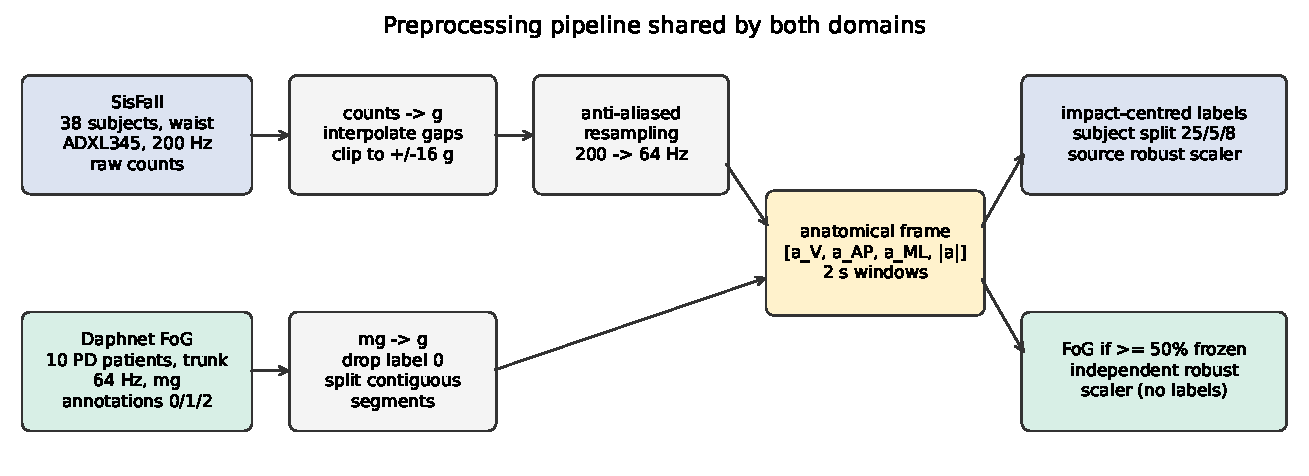
\includegraphics[width=\textwidth]{fig01_pipeline}
\caption{Preprocessing shared by both domains. Only the population and the target event differ
between the two branches.}
\label{fig:pipeline}
\end{figure}

\section{Exploratory analysis}
\label{sec:eda}

\paragraph{Axis identification.} \Cref{fig:axes} confirms the data-driven frame: walking puts
$0.97\,g$ on the vertical axis, and the static acceleration after a fall moves to $a_{AP}=-0.60\,g$
for forward falls and $+0.83\,g$ for backward falls, i.e.\ prone and supine, as the sign convention
predicts. The small negative AP offset during walking ($-0.2\,g$) shows that the SisFall logger was
tilted on the belt by roughly 12 degrees, a reminder that ``the waist'' is not one orientation.

\begin{figure}[ht]
\centering
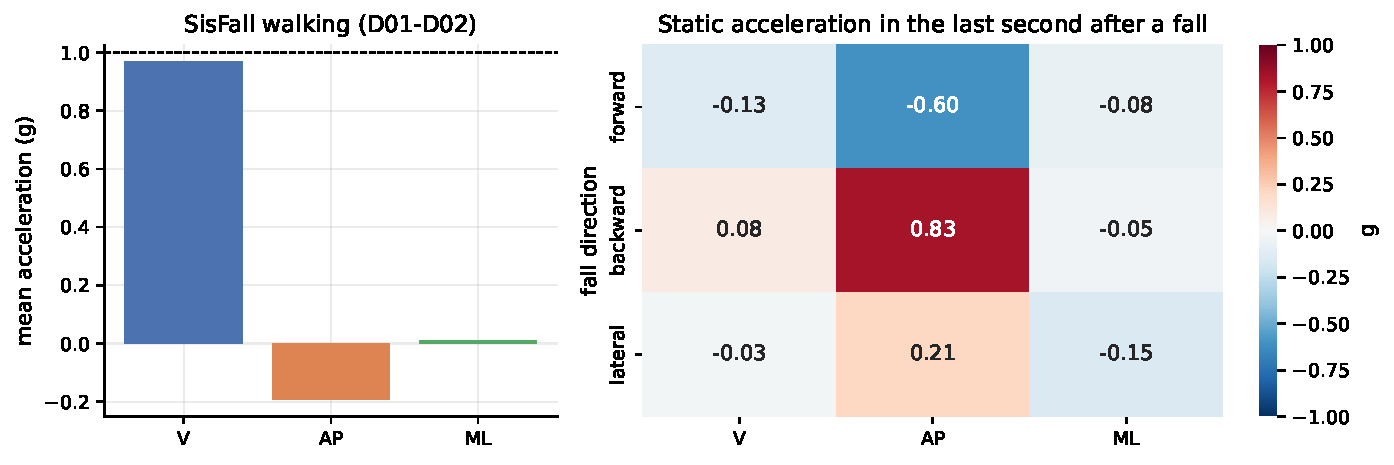
\includegraphics[width=0.95\textwidth]{fig03_axis_identification}
\caption{Left: mean acceleration per anatomical axis during SisFall walking. Right: static acceleration
in the last second of fall trials, grouped by the fall direction given in the dataset documentation.}
\label{fig:axes}
\end{figure}

\paragraph{Signal morphology.} A SisFall fall is a short, violent transient followed by rest in a new
orientation (\Cref{fig:sisfall-signal}). At the trunk, a Daphnet freeze looks very different: the
gait rhythm becomes irregular and small, fast oscillations appear, but nothing comparable to an
impact occurs (\Cref{fig:daphnet-signal}). The ankle shows the trembling more clearly than the trunk,
which is why the freeze index is usually computed at the shank.

\begin{figure}[ht]
\centering
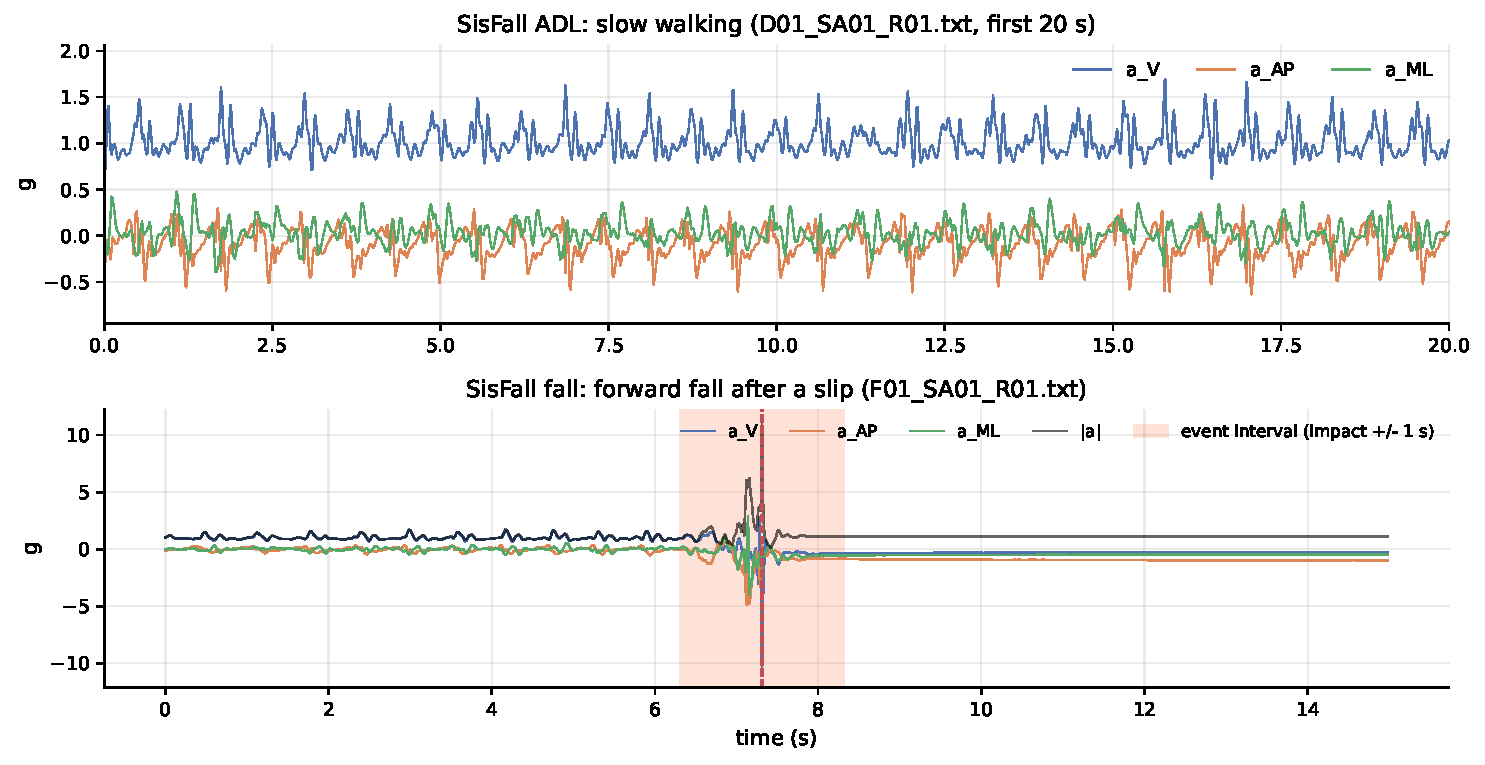
\includegraphics[width=\textwidth]{fig04_sisfall_signals}
\caption{SisFall in the common frame. Top: slow walking. Bottom: forward fall after a slip; the shaded
band is the event interval used for labelling and the dashed line the detected impact.}
\label{fig:sisfall-signal}
\end{figure}

\begin{figure}[ht]
\centering
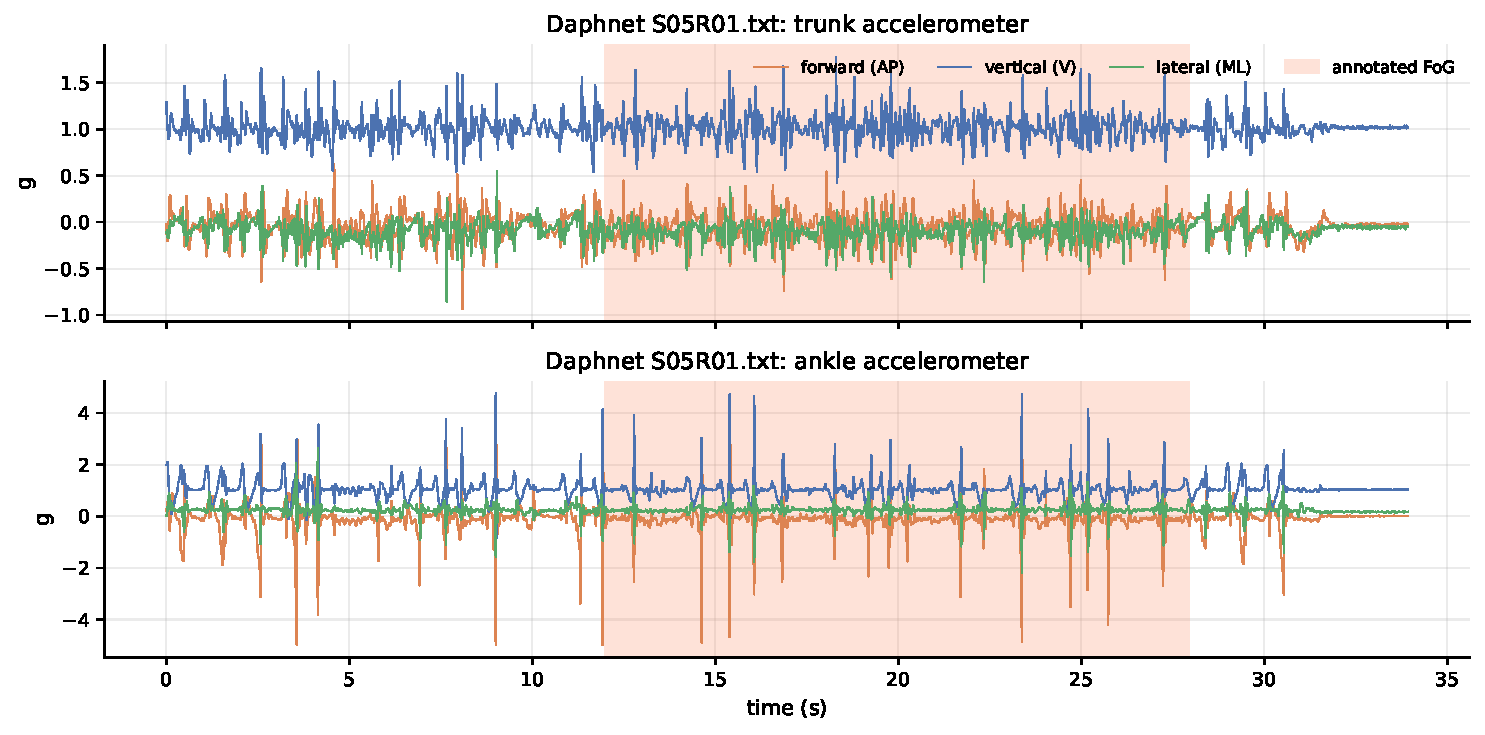
\includegraphics[width=\textwidth]{fig05_daphnet_signals}
\caption{Daphnet recording with the longest freezing episode, trunk (used by the models) and ankle
(for reference). The shaded band is the clinical FoG annotation.}
\label{fig:daphnet-signal}
\end{figure}

\paragraph{Descriptors and spectra.} \Cref{fig:descriptors} and \Cref{tab:mannwhitney} quantify the
difference. A fall window has a median peak of $5.6\,g$ and a $|a|$ standard deviation thirteen times
that of ADL (rank-biserial $r=0.94$ and $0.82$). FoG windows differ from Parkinsonian walking much less:
a factor of two in $|a|$ variability, $0.2\,g$ in peak and $+0.3$ in log freeze index, all with moderate
effect sizes ($r=0.33$--$0.37$). The largest difference between the two \emph{normal} classes, healthy
ADL and Parkinsonian walking, is spectral: the freeze index is higher in Daphnet ($r=0.42$) while
amplitudes are almost identical. In the frequency domain
(\Cref{fig:psd}), falls raise the power at every frequency by about two orders of magnitude, while FoG
adds a bump between 3 and 8\,Hz. The positive classes of the two domains barely overlap: in raw
window statistics, falls form an isolated cluster, whereas FoG windows share most of their
neighbourhoods with walking windows (\Cref{fig:tsne-raw}). This is the first piece of evidence that the transfer problem is dominated by
concept shift.

\begin{figure}[ht]
\centering
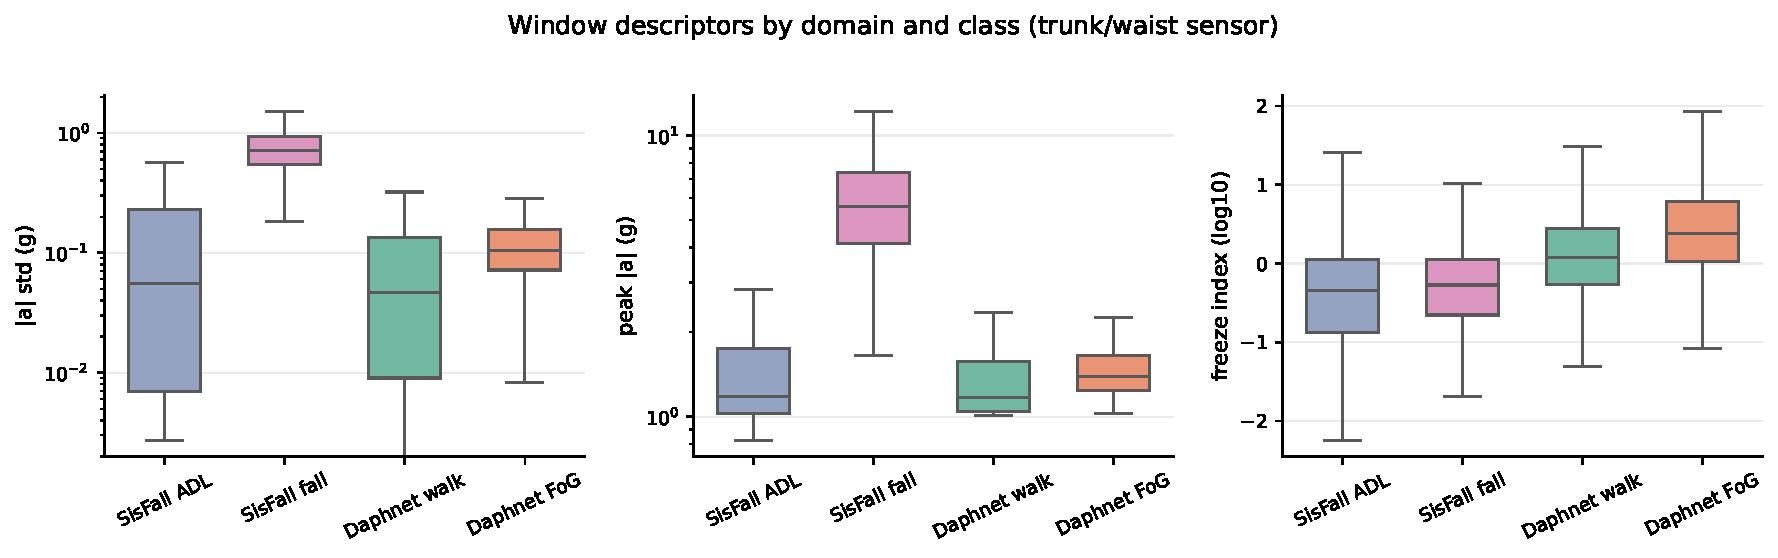
\includegraphics[width=\textwidth]{fig06_window_descriptors}
\caption{Window descriptors (random subsets of up to 6{,}000 windows per group; outliers hidden).
The freeze index is computed on the AP axis.}
\label{fig:descriptors}
\end{figure}

\begin{table}[ht]
\centering
\small
\caption{Window descriptors: medians and Mann--Whitney rank-biserial effect size $r$ (all $p<10^{-10}$ unless stated).}
\label{tab:mannwhitney}
\begin{adjustbox}{max width=\textwidth}
\begin{tabular}{llrrr}
\toprule
Comparison (A vs B) & Descriptor & Median A & Median B & $r$ \\
\midrule
SisFall ADL vs SisFall fall & $|a|$ std (g) & 0.055 & 0.714 & 0.82 \\
 & peak $|a|$ (g) & 1.179 & 5.575 & 0.94 \\
 & freeze index (log10) & -0.338 & -0.273 & 0.09 ($p=2.5e-08$) \\
Daphnet walk vs Daphnet FoG & $|a|$ std (g) & 0.047 & 0.104 & 0.37 \\
 & peak $|a|$ (g) & 1.172 & 1.389 & 0.34 \\
 & freeze index (log10) & 0.077 & 0.381 & 0.33 \\
SisFall ADL vs Daphnet walk & $|a|$ std (g) & 0.055 & 0.047 & -0.04 ($p=2.1e-05$) \\
 & peak $|a|$ (g) & 1.179 & 1.172 & 0.01 ($p=5.9e-01$) \\
 & freeze index (log10) & -0.338 & 0.077 & 0.42 \\
\bottomrule
\end{tabular}
\end{adjustbox}
\end{table}

\begin{figure}[ht]
\centering
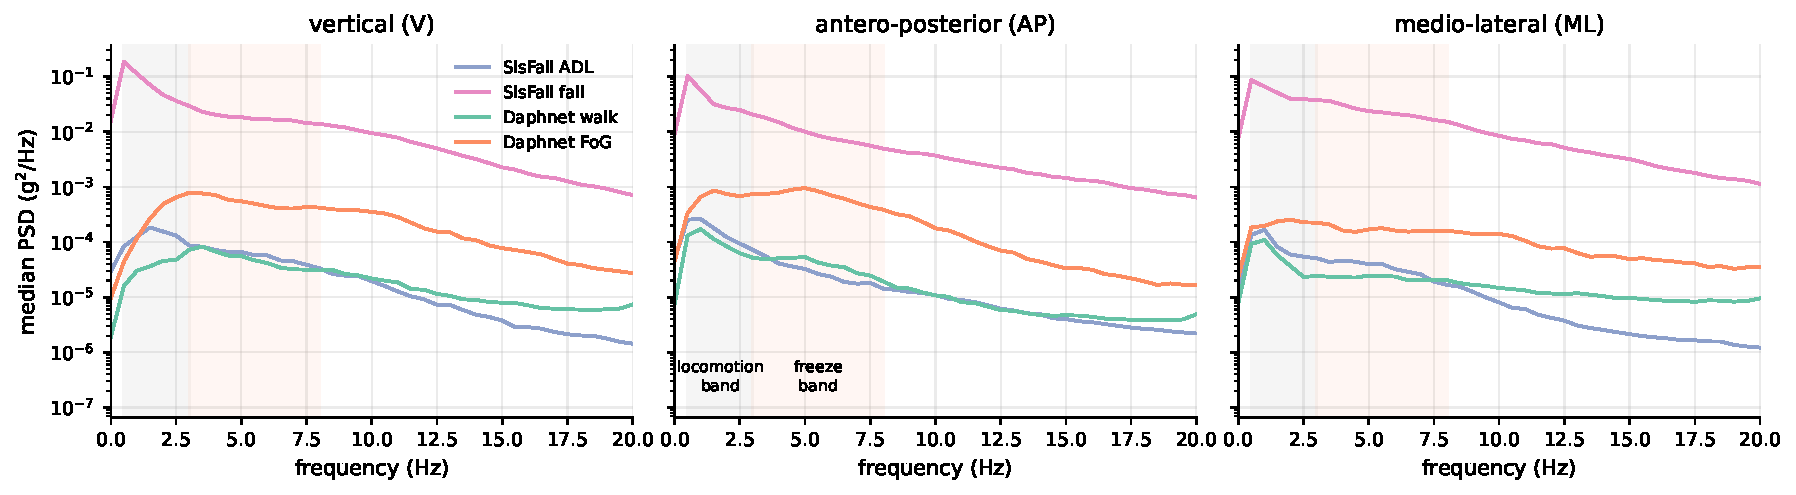
\includegraphics[width=\textwidth]{fig07_power_spectra}
\caption{Median Welch power spectral density per group and axis (mean removed per window). Grey:
locomotion band; orange: freeze band.}
\label{fig:psd}
\end{figure}

\begin{figure}[ht]
\centering
\begin{subfigure}{0.48\textwidth}
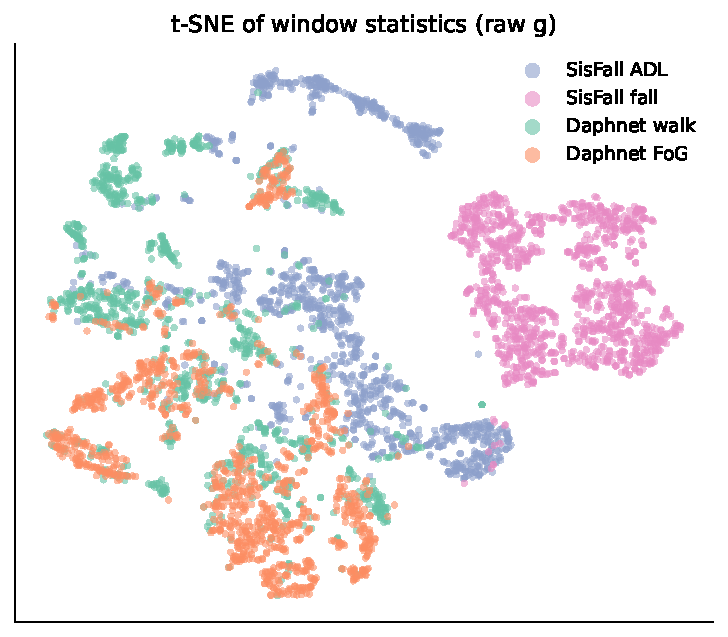
\includegraphics[width=\textwidth]{fig10_tsne_raw_features}
\caption{t-SNE of window statistics.}
\label{fig:tsne-raw}
\end{subfigure}\hfill
\begin{subfigure}{0.48\textwidth}
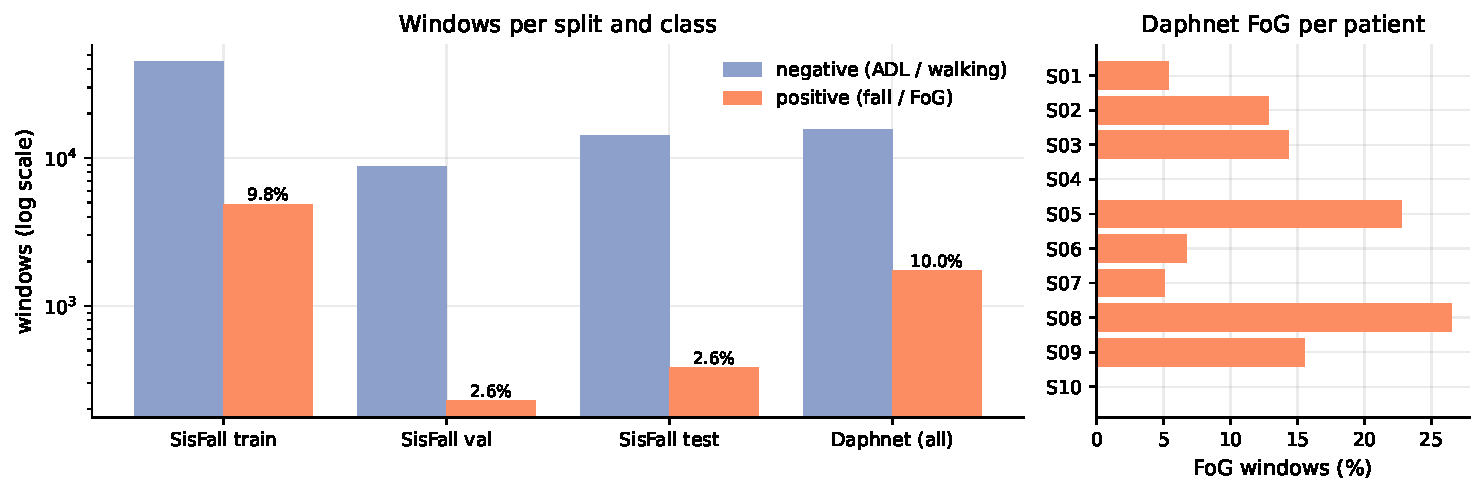
\includegraphics[width=\textwidth]{fig02_class_balance}
\caption{Class balance per split.}
\end{subfigure}
\caption{Left: hand-crafted window statistics (per-channel mean, standard deviation, percentiles and
the descriptors above) embedded with t-SNE. Right: windows per split and class (log scale) and FoG
prevalence per Daphnet patient.}
\end{figure}

\paragraph{Amplitude distributions and scaling.} Raw per-channel distributions of healthy ADL and
Parkinsonian walking are already close (\Cref{fig:amplitude}, left), because both are dominated by
upright posture. Scaling with source statistics leaves Daphnet much narrower than SisFall on the
vertical and magnitude channels; scaling each domain with its own statistics widens Daphnet to unit
inter-quartile range, which brings the walking distributions closer but also amplifies the small
FoG oscillations. Daphnet values are stored with a resolution of about 10\,mg against 3.9\,mg for the
ADXL345, another (minor) difference between the sensors.

\begin{figure}[ht]
\centering
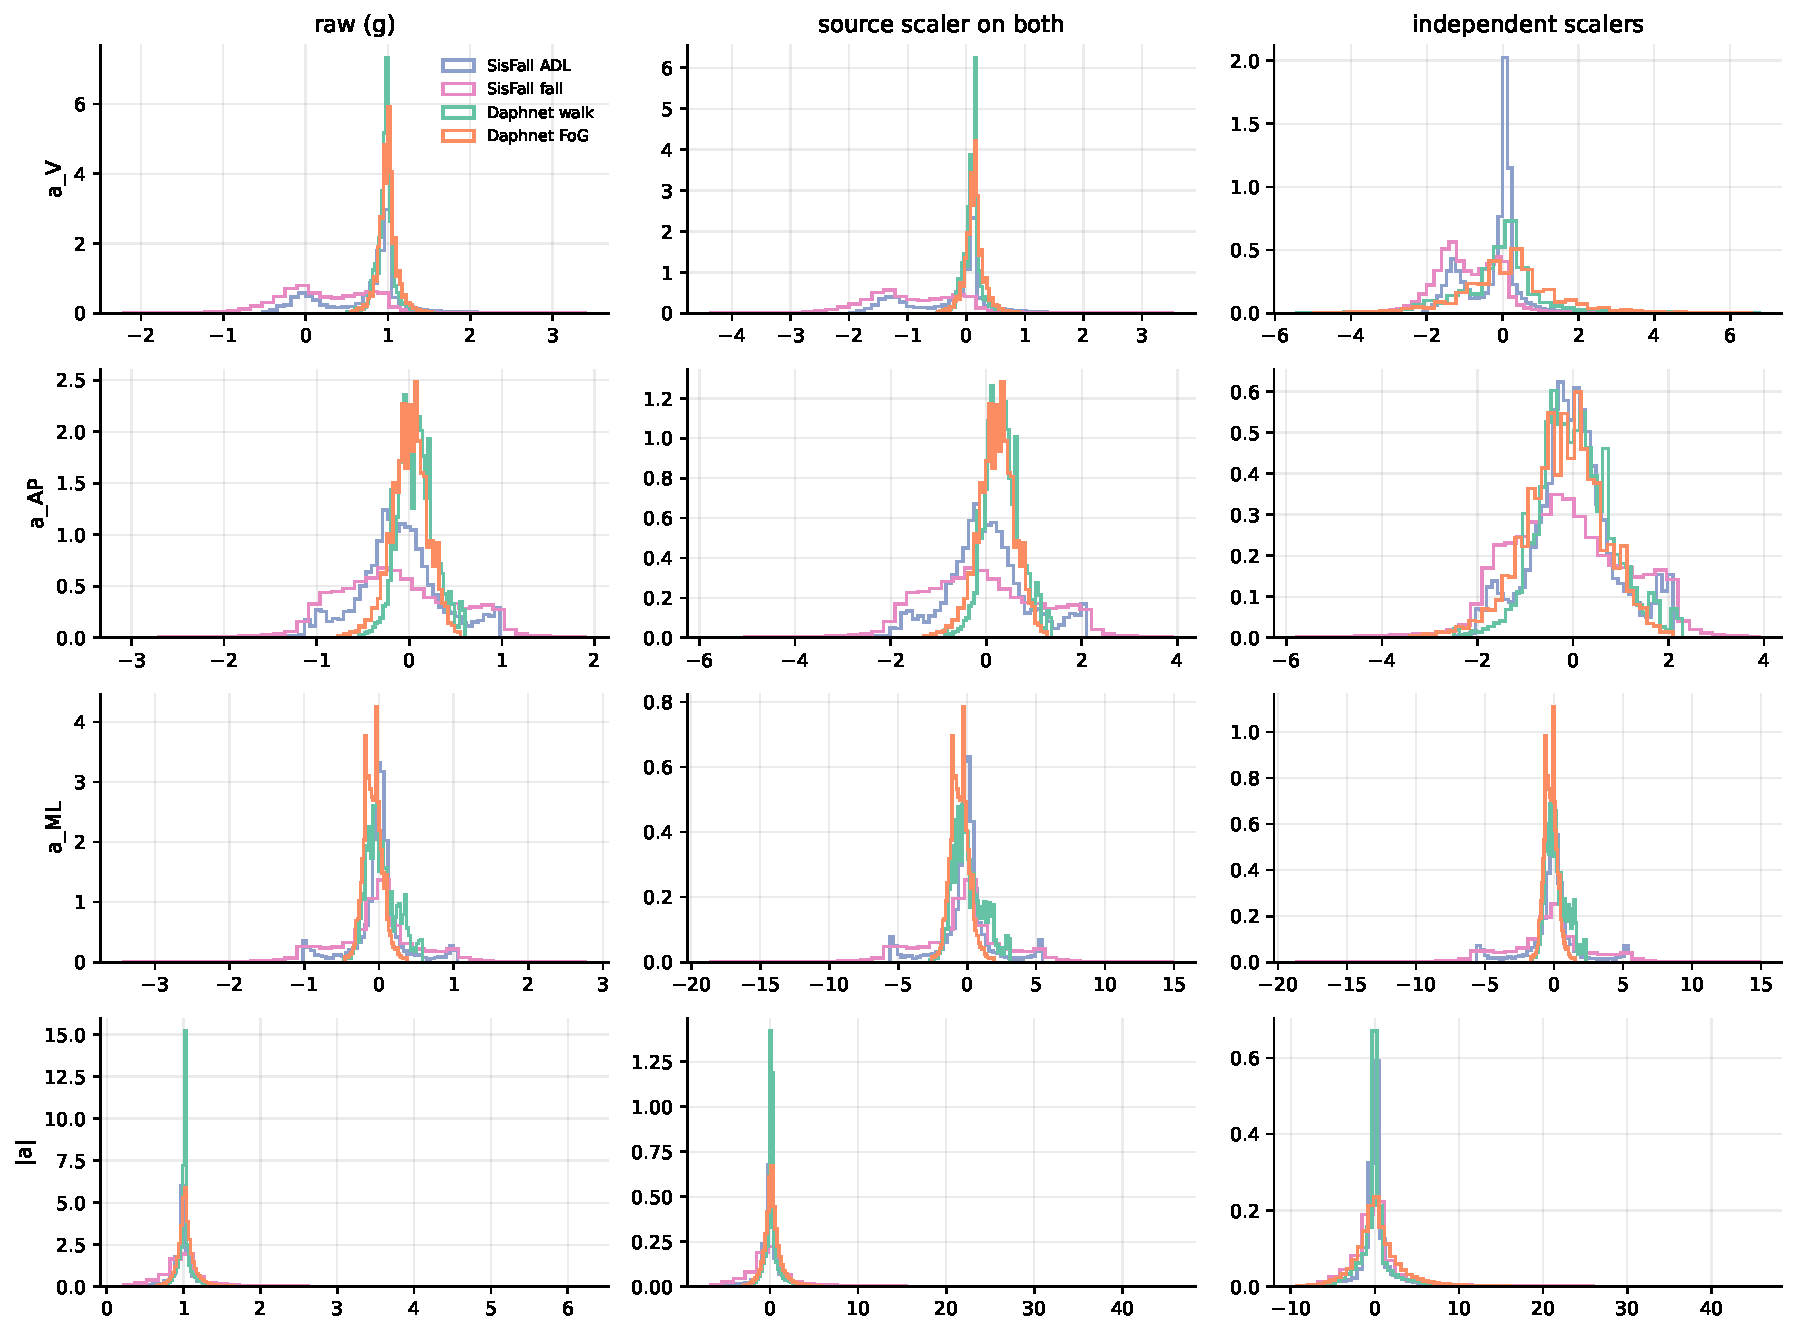
\includegraphics[width=\textwidth]{fig08_amplitude_distributions}
\caption{Per-channel sample distributions in raw units, with the source scaler applied to both domains,
and with independent per-domain scalers.}
\label{fig:amplitude}
\end{figure}

\section{Implementation}

Everything is implemented in PyTorch \parencite{paszke2019pytorch} and executed end to end in six
Jupyter notebooks (data preparation, exploratory analysis, hyper-parameter search, training and
zero-shot evaluation, target adaptation, shift analysis). Shared components (models, training loop,
metrics) live in a small \texttt{src} package so that the notebooks call identical code. Network
training (notebooks 03--05) ran on one NVIDIA T4 GPU; preprocessing, inference from the saved
checkpoints and all analyses also run on a two-core CPU, where they reproduce the reported metrics.
The training cost per epoch is given in \Cref{tab:hparams}.
Each checkpoint stores the weights together with the configuration, the scaler statistics and the
validation threshold, so it is self-contained for inference.

\chapter{Experiments and Results}
\label{ch:results}

All numbers in this chapter are produced by notebooks 03--07 and stored in
\texttt{results/metrics}. Unless stated otherwise, results are mean $\pm$ standard deviation over three
seeds, and Daphnet inputs are normalised with independent, label-free domain statistics.

\section{Model selection on a saturated source task}
\label{sec:selection}

The first surprise came before any transfer experiment. With impact-centred labels, fall detection
on SisFall is close to solved: 18 of the 24 configurations in the search reach a validation AUPRC of
at least 0.999, and the selected models of every architecture reach 1.000 within two or three epochs (\Cref{fig:curves},
\Cref{fig:hpsearch}). AUPRC therefore cannot rank configurations or checkpoints, so we break ties with
the unweighted validation cross-entropy, which keeps decreasing for several more epochs. The selected
models are listed in \Cref{tab:hparams}. The search picked a two-layer bidirectional network for both
recurrent families, and the GRU ended up with the smallest model of the four (26k parameters).

\begin{table}[ht]
\centering
\small
\caption{Configurations selected on SisFall validation, trainable parameters, mean epochs to the selected checkpoint and training time per epoch on one NVIDIA T4 GPU.}
\label{tab:hparams}
\begin{adjustbox}{max width=\textwidth}
\begin{tabular}{lp{6.3cm}rrrr}
\toprule
Model & Configuration & lr & Params & Best ep. & s/epoch \\
\midrule
CNN-1D & width 32, kernel 7, dropout 0.5 & 3e-3 & 36,289 & 5.7 & 2 \\
LSTM & hidden 64, 2 layers, bidirectional, dropout 0.3 & 1e-3 & 135,425 & 8.0 & 4 \\
GRU & hidden 32, 2 layers, bidirectional, dropout 0.1 & 3e-3 & 26,241 & 9.7 & 2 \\
Transformer & $d=64$, 2 layers, patch 8, dropout 0.2 & 3e-3 & 70,401 & 7.3 & 3 \\
\bottomrule
\end{tabular}
\end{adjustbox}
\end{table}

Among the 18 saturated configurations, Daphnet AUROC ranges from 0.43 to 0.69 and is unrelated to
validation AUPRC (Spearman $\rho=0.23$, $p=0.37$). It is moderately related to validation loss
($\rho=-0.49$, $p=0.04$): better-calibrated source models transfer slightly better, which supports the
tie-breaking rule but is far from a reliable selection signal. An oracle that picked the
configuration with the best Daphnet AUROC would have changed the choice for the CNN only (0.54 $\to$
0.69 in the search setting) and for the LSTM marginally (0.51 $\to$ 0.52). We do not use these oracle
choices anywhere else.

\section{E1: in-domain fall detection}
\label{sec:e1}

\Cref{tab:sisfall} and the left panels of \Cref{fig:roc} report results on the eight held-out SisFall
subjects (381 fall windows, 14{,}173 non-fall windows, i.e.\ 3.9 hours of activity). The four
architectures are within two points of each other on every metric. The recurrent models have the
highest AUROC (0.999) and the fewest false alarms (0.7--0.8 per hour of activity). The CNN-1D has the
highest recall (0.980) but a lower AUROC (0.987), caused by a handful of falls that receive very low
scores; its seed-to-seed variability is also the largest (thresholds selected on validation range from
0.12 to 0.94). The Transformer misses the most falls (recall 0.959, about 16 of 381 per seed against 8
for the recurrent models). Subject-level bootstrap intervals overlap for all models (\Cref{tab:ci}).
In short, on the source task all four architectures are excellent, and the data do not support
ranking them.

\begin{table}[ht]
\centering
\footnotesize
\caption{In-domain fall detection on the eight SisFall test subjects (mean $\pm$ std over three seeds). Recall, specificity, F$_1$ and false alarms per hour (FA/h, one negative window per second of activity) use the threshold selected on validation. Best mean in bold.}
\label{tab:sisfall}
\setlength{\tabcolsep}{4pt}
\begin{adjustbox}{max width=\textwidth}
\begin{tabular}{lcccccc}
\toprule
Model & AUROC & AUPRC & Recall & Spec. & F$_1$ & FA/h \\
\midrule
CNN-1D & 0.987 $\pm$ 0.003 & 0.980 $\pm$ 0.002 & \textbf{0.980 $\pm$ 0.002} & \textbf{1.000 $\pm$ 0.000} & 0.982 $\pm$ 0.006 & 1.5 $\pm$ 1.1 \\
LSTM & \textbf{0.999 $\pm$ 0.000} & 0.990 $\pm$ 0.002 & 0.977 $\pm$ 0.010 & \textbf{1.000 $\pm$ 0.000} & \textbf{0.985 $\pm$ 0.005} & 0.8 $\pm$ 0.0 \\
GRU & \textbf{0.999 $\pm$ 0.000} & \textbf{0.992 $\pm$ 0.002} & 0.977 $\pm$ 0.003 & \textbf{1.000 $\pm$ 0.000} & \textbf{0.985 $\pm$ 0.002} & \textbf{0.7 $\pm$ 0.1} \\
Transformer & 0.998 $\pm$ 0.001 & 0.984 $\pm$ 0.005 & 0.959 $\pm$ 0.010 & \textbf{1.000 $\pm$ 0.000} & 0.974 $\pm$ 0.008 & 0.9 $\pm$ 0.5 \\
\bottomrule
\end{tabular}
\end{adjustbox}
\end{table}

\begin{figure}[ht]
\centering
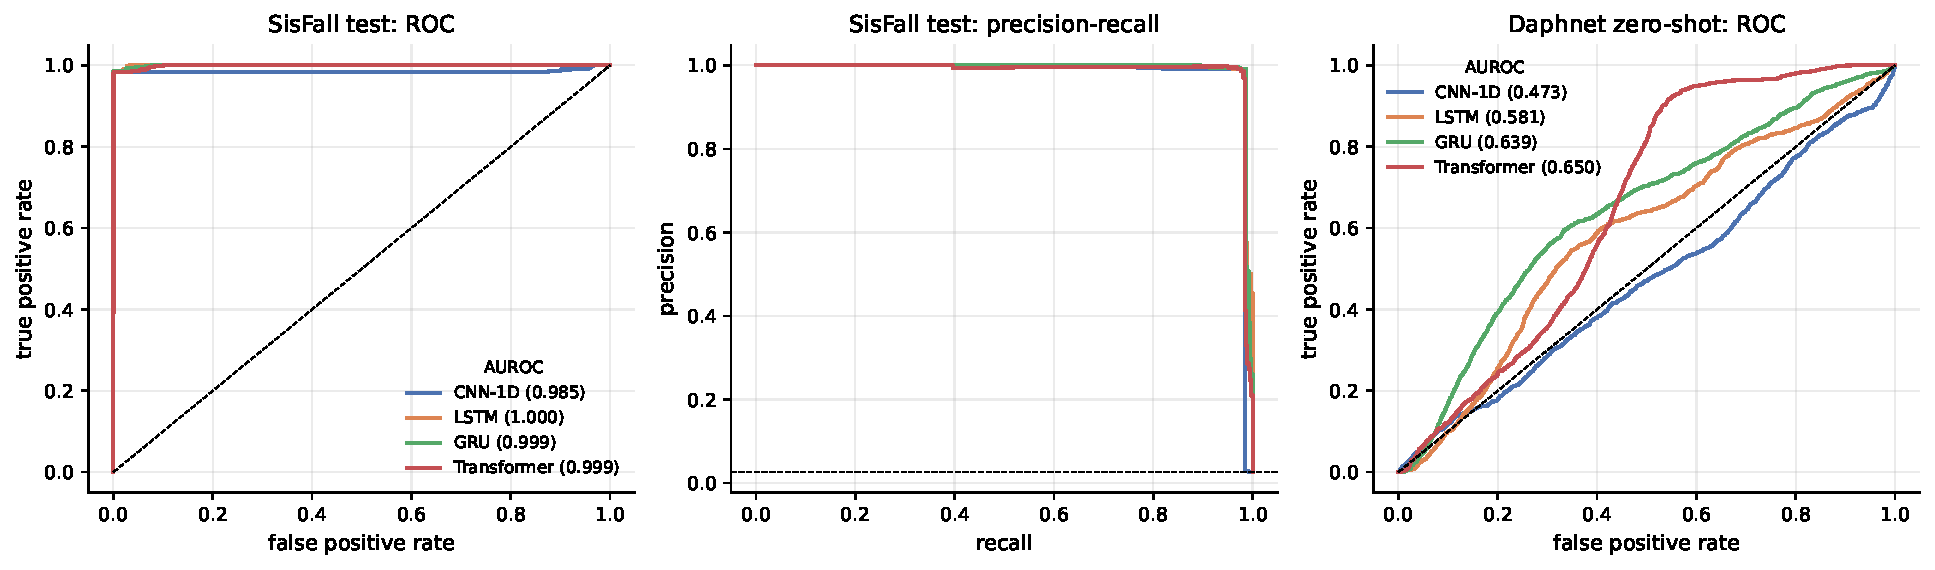
\includegraphics[width=\textwidth]{fig14_roc_pr_curves}
\caption{ROC and precision-recall curves of the seed-averaged scores. Left and centre: SisFall test
subjects. Right: zero-shot transfer to Daphnet.}
\label{fig:roc}
\end{figure}

\section{E2: zero-shot transfer to freezing of gait}
\label{sec:e2}

\paragraph{Ranking.} On Daphnet, AUROC falls to 0.49--0.63 (\Cref{tab:zeroshot}); AUPRC is 0.10--0.14
for a prevalence of 0.10. Averaging the three seeds gives 0.47 (CNN-1D), 0.58 (LSTM), 0.64 (GRU) and
0.65 (Transformer). With patients as the resampling unit, only the Transformer's 95\% interval excludes
chance, [0.55, 0.73] (\Cref{tab:ci}). The ROC curves (\Cref{fig:roc}, right) show that whatever
signal exists sits at mid-range false-positive rates, which is useless for an alarm.

\begin{table}[ht]
\centering
\footnotesize
\caption{Zero-shot transfer to Daphnet (all 17 recordings, independent domain statistics, SisFall-validated threshold). Positives are FoG windows. Best mean in bold.}
\label{tab:zeroshot}
\setlength{\tabcolsep}{4pt}
\begin{adjustbox}{max width=\textwidth}
\begin{tabular}{lcccccc}
\toprule
Model & AUROC & AUPRC & Recall & Spec. & F$_1$ & FA/h \\
\midrule
CNN-1D & 0.491 $\pm$ 0.056 & 0.104 $\pm$ 0.008 & \textbf{0.009 $\pm$ 0.008} & 0.994 $\pm$ 0.003 & \textbf{0.017 $\pm$ 0.015} & 23.3 $\pm$ 12.2 \\
LSTM & 0.587 $\pm$ 0.032 & 0.124 $\pm$ 0.021 & 0.001 $\pm$ 0.001 & 0.996 $\pm$ 0.000 & 0.001 $\pm$ 0.001 & 13.6 $\pm$ 0.9 \\
GRU & \textbf{0.631 $\pm$ 0.042} & \textbf{0.143 $\pm$ 0.023} & 0.000 $\pm$ 0.000 & \textbf{0.997 $\pm$ 0.001} & 0.000 $\pm$ 0.000 & \textbf{11.8 $\pm$ 5.1} \\
Transformer & 0.620 $\pm$ 0.036 & 0.128 $\pm$ 0.009 & 0.000 $\pm$ 0.000 & 0.995 $\pm$ 0.002 & 0.000 $\pm$ 0.001 & 17.1 $\pm$ 7.8 \\
\bottomrule
\end{tabular}
\end{adjustbox}
\end{table}
\begin{table}[ht]
\centering
\small
\caption{AUROC of the seed-averaged scores with 95\% subject-level bootstrap intervals.}
\label{tab:ci}
\begin{adjustbox}{max width=\textwidth}
\begin{tabular}{lcc}
\toprule
Model & SisFall test & Daphnet zero-shot \\
\midrule
CNN-1D & 0.985 [0.961, 1.000] & 0.473 [0.407, 0.546] \\
LSTM & 1.000 [0.999, 1.000] & 0.581 [0.381, 0.711] \\
GRU & 0.999 [0.998, 1.000] & 0.639 [0.458, 0.765] \\
Transformer & 0.999 [0.997, 1.000] & 0.650 [0.548, 0.733] \\
\bottomrule
\end{tabular}
\end{adjustbox}
\end{table}

\paragraph{Operating point.} At the threshold validated on SisFall, the detectors almost never fire on
Daphnet. Recall is below 1\% for every model, and the GRU flags none of the 1{,}734 FoG windows in any
seed (\Cref{fig:cm}). The score distributions explain why: walking and FoG windows both receive
log-odds between $-10$ and $-4$, four (CNN-1D) to ten (recurrent models, Transformer) units below the decision threshold (\Cref{fig:scores}).
This silence is informative in itself. With file-level labels, the pre-fall walking of SisFall
fall trials would be a positive example and irregular gait could easily look like a fall; with an
ankle sensor fed where the network expects a waist sensor, the inputs alone would push the scores up.
Either confounder could produce the opposite behaviour, an alarm on most Parkinsonian walking. Once
the event is defined as the impact and the sensors are matched, the detectors become very specific
to what they were taught.

\paragraph{False alarms still increase.} Even so, the false-positive rate on Daphnet walking is 0.3--0.7\%,
which corresponds to 12--23 false alarms per hour of walking, 15 to 18 times the rate measured on
healthy and elderly ADL. Covariate shift alone, without any FoG, degrades specificity by more than an
order of magnitude.

\begin{figure}[ht]
\centering
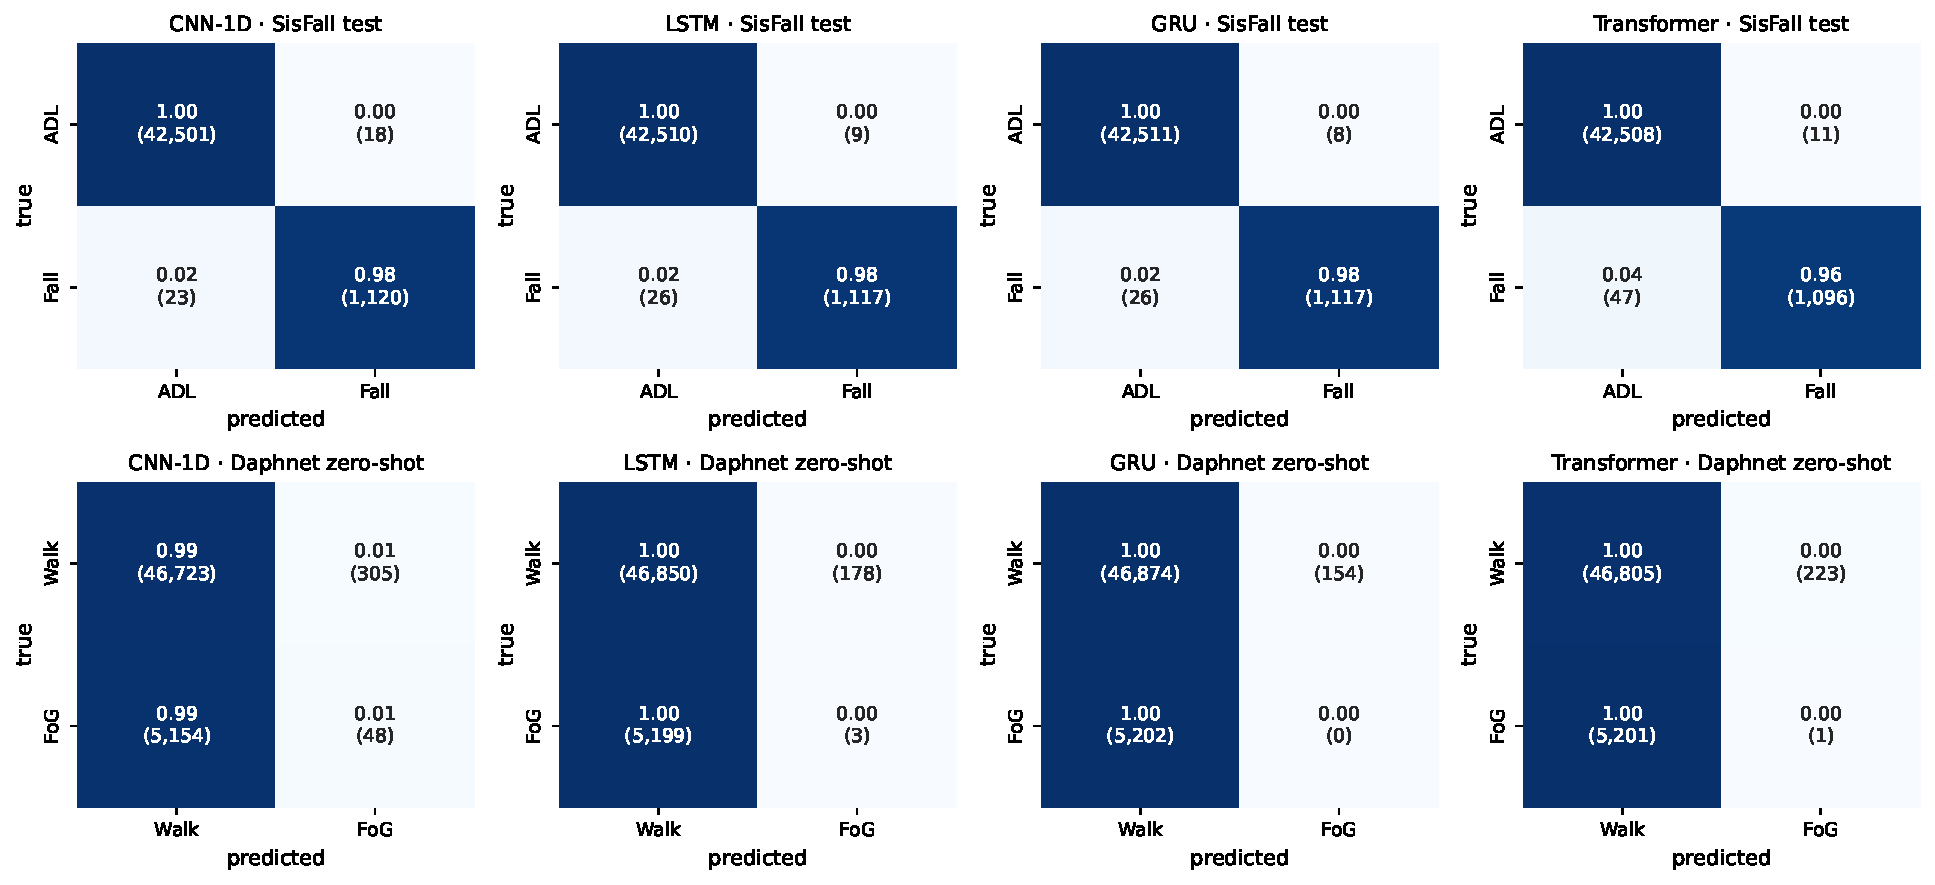
\includegraphics[width=\textwidth]{fig15_confusion_matrices}
\caption{Confusion matrices summed over the three seeds. Top: SisFall test. Bottom: Daphnet zero-shot.
Rows are normalised; counts in brackets.}
\label{fig:cm}
\end{figure}

\begin{figure}[ht]
\centering
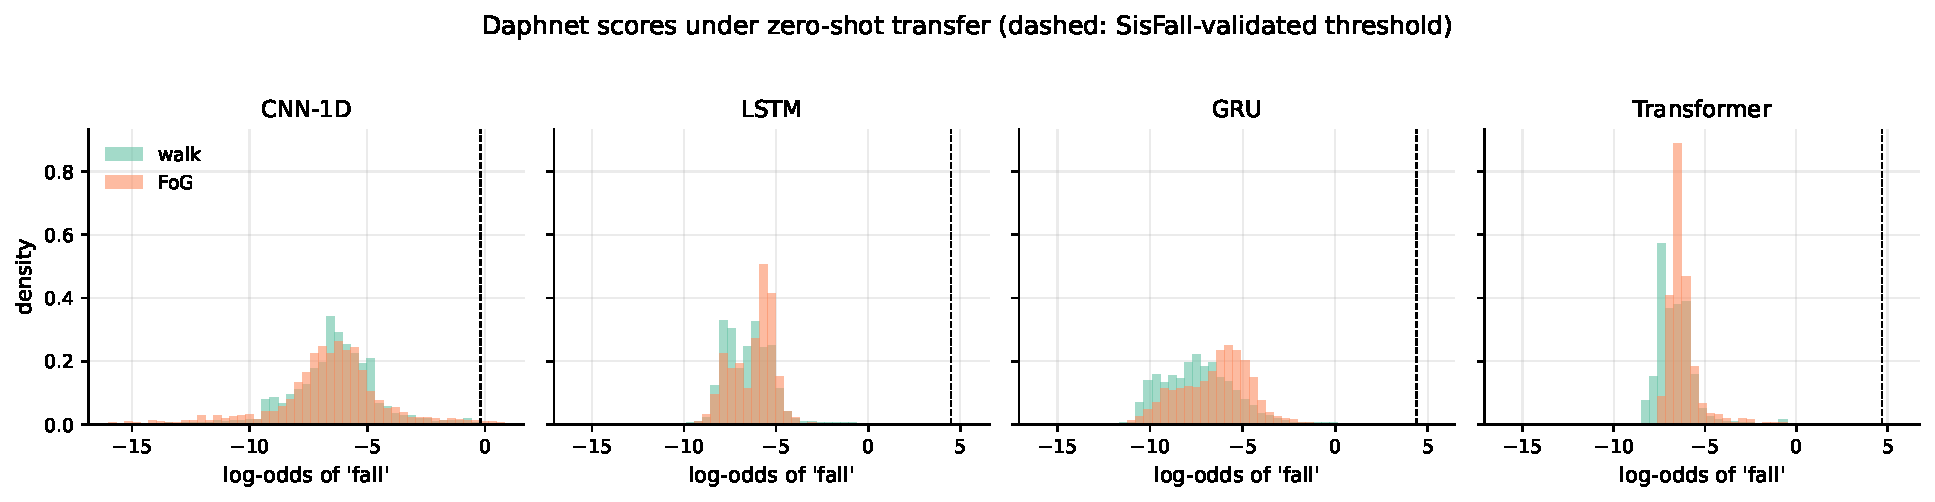
\includegraphics[width=\textwidth]{fig17_daphnet_score_distributions}
\caption{Seed-averaged Daphnet scores, shown as log-odds because almost all probabilities are close to
zero. The dashed line is the SisFall-validated threshold.}
\label{fig:scores}
\end{figure}

\paragraph{A training-free reference.} Two scores computed directly from each window, with no learning,
do better than every network: the freeze index on the trunk AP axis reaches an AUROC of 0.663, and
the standard deviation of $|a|$ reaches 0.682. At the trunk, FoG windows are on average more agitated
than the walking class, which also contains standing and turning. A fall detector could in principle
exploit that, but its scores carry less information about FoG than a single energy statistic.

\paragraph{Patients.} Per-patient AUROC ranges from 0.26 to 0.85 (\Cref{fig:perpatient}). The recurrent
models and the Transformer rank FoG above walking for S01, S02, S03 and S05 (0.60--0.85) and below it
for S06 and S08 (0.27--0.49). The CNN-1D shows almost the mirror pattern. A pooled AUROC around 0.6
thus hides patient-specific behaviour in both directions.

\begin{figure}[ht]
\centering
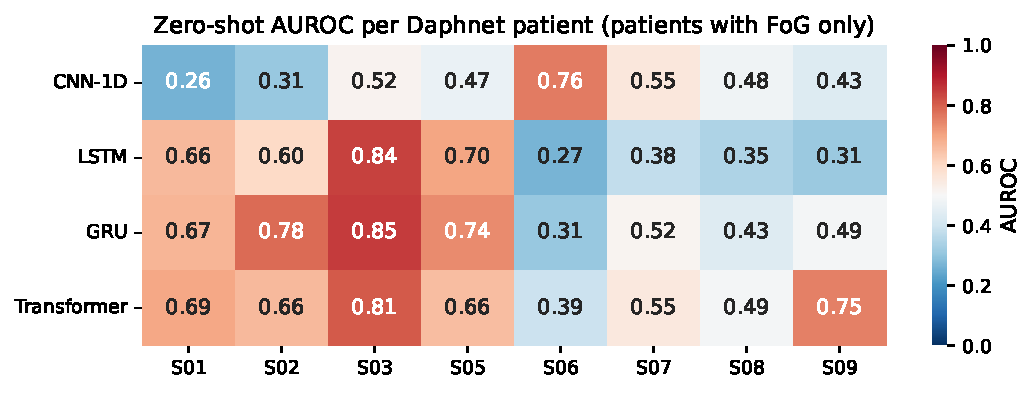
\includegraphics[width=0.9\textwidth]{fig18_per_patient_auroc}
\caption{Zero-shot AUROC per Daphnet patient (seed-averaged scores; S04 and S10 have no FoG).}
\label{fig:perpatient}
\end{figure}

\section{Does normalisation fix it?}
\label{sec:ablation}

\Cref{tab:ablation} and \Cref{fig:ablation} compare the three label-free normalisations of the target.
No variant brings any model close to the training-free reference. Re-estimating the statistics on
Daphnet helps the recurrent models and the Transformer slightly (GRU $+0.06$, LSTM $+0.04$, Transformer
$+0.02$) and hurts the CNN-1D ($-0.13$); per-patient statistics fall in between. First- and
second-order covariate correction at the input is not the bottleneck.

\begin{table}[ht]
\centering
\footnotesize
\caption{Zero-shot Daphnet results under three label-free normalisations of the target inputs: AUROC (mean $\pm$ std over seeds) and, in brackets, recall / false-positive rate at the SisFall threshold.}
\label{tab:ablation}
\begin{adjustbox}{max width=\textwidth}
\begin{tabular}{lccc}
\toprule
Model & Source statistics & Domain statistics & Subject statistics \\
\midrule
CNN-1D & 0.621 $\pm$ 0.064 (0.0\% / 0.2\%) & 0.491 $\pm$ 0.056 (0.9\% / 0.6\%) & 0.528 $\pm$ 0.042 (0.8\% / 2.0\%) \\
LSTM & 0.547 $\pm$ 0.064 (0.0\% / 0.1\%) & 0.587 $\pm$ 0.032 (0.1\% / 0.4\%) & 0.554 $\pm$ 0.031 (0.0\% / 0.4\%) \\
GRU & 0.571 $\pm$ 0.051 (0.0\% / 0.1\%) & 0.631 $\pm$ 0.042 (0.0\% / 0.3\%) & 0.604 $\pm$ 0.027 (0.0\% / 0.3\%) \\
Transformer & 0.603 $\pm$ 0.087 (0.0\% / 0.0\%) & 0.620 $\pm$ 0.036 (0.0\% / 0.5\%) & 0.596 $\pm$ 0.054 (0.0\% / 0.7\%) \\
\bottomrule
\end{tabular}
\end{adjustbox}
\end{table}

\begin{figure}[ht]
\centering
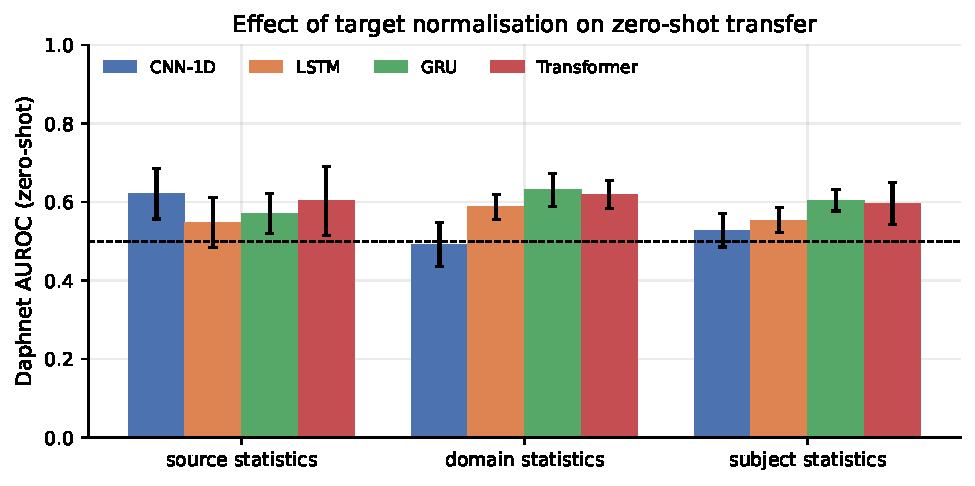
\includegraphics[width=0.75\textwidth]{fig13_normalisation_ablation}
\caption{Zero-shot Daphnet AUROC under three label-free normalisations (mean $\pm$ std over seeds).}
\label{fig:ablation}
\end{figure}

\section{E3: what target labels buy, and whether fall pre-training helps}
\label{sec:e3}

\Cref{tab:adaptation} and \Cref{fig:adaptation} give the target-domain references under 5-fold
patient-grouped cross-validation. Trained from scratch on six patients, the CNN-1D reaches an AUROC of
0.786, the Transformer 0.776 and the GRU 0.769, with large fold-to-fold variation ($\pm$0.15--0.19)
that reflects the heterogeneity between patients. The bidirectional LSTM is unstable with this little
data (0.608 $\pm$ 0.251). With only two training patients, the CNN-1D (0.714) and the Transformer
(0.696) degrade gracefully, while the recurrent models fall to chance. This trunk-only, 2\,s-window
ceiling of roughly 0.78 puts the zero-shot numbers in perspective: the best zero-shot model covers
about half of the distance between chance and this modest supervised ceiling, and the training-free
freeze index covers more.

\begin{table}[ht]
\centering
\footnotesize
\caption{Daphnet AUROC / AUPRC on held-out patients, 5-fold patient-grouped cross-validation (mean $\pm$ std over folds). FoG prevalence is 10\%, the AUPRC of a random detector.}
\label{tab:adaptation}
\setlength{\tabcolsep}{3pt}
\begin{adjustbox}{max width=\textwidth}
\begin{tabular}{lcccc}
\toprule
Setting & CNN-1D & LSTM & GRU & Transformer \\
\midrule
Zero-shot (no target labels) & 0.395$\pm$0.220 / 0.114 & 0.549$\pm$0.235 / 0.123 & 0.641$\pm$0.199 / 0.155 & 0.687$\pm$0.128 / 0.163 \\
Scratch, 2 patients & 0.714$\pm$0.123 / 0.238 & 0.351$\pm$0.256 / 0.104 & 0.548$\pm$0.255 / 0.195 & 0.696$\pm$0.153 / 0.215 \\
Fine-tuned, 2 patients & 0.617$\pm$0.144 / 0.161 & 0.435$\pm$0.170 / 0.089 & 0.588$\pm$0.167 / 0.132 & 0.668$\pm$0.195 / 0.179 \\
Scratch, 6 patients & 0.786$\pm$0.147 / 0.387 & 0.608$\pm$0.251 / 0.202 & 0.769$\pm$0.189 / 0.373 & 0.776$\pm$0.178 / 0.350 \\
Fine-tuned, 6 patients & 0.727$\pm$0.175 / 0.302 & 0.437$\pm$0.173 / 0.099 & 0.700$\pm$0.201 / 0.223 & 0.732$\pm$0.225 / 0.300 \\
\bottomrule
\end{tabular}
\end{adjustbox}
\end{table}

Fine-tuning from the SisFall weights does not help (\Cref{tab:pretrain}). With six training patients,
pre-training lowers the mean AUROC for all four architectures (by 0.04 to 0.17) and improves only one
fold out of five in each case. With two patients the picture is mixed (two small gains for the
recurrent models, two losses). None of the differences is significant with five folds (Wilcoxon
$p\geq0.125$), but the direction is consistent: the fall representation is a worse starting point
than random initialisation. This is negative transfer.

\begin{table}[ht]
\centering
\small
\caption{Effect of SisFall pre-training on Daphnet AUROC: mean difference (fine-tuned $-$ scratch), folds improved out of five, and Wilcoxon signed-rank $p$ (five folds, so $p\ge0.0625$).}
\label{tab:pretrain}
\begin{adjustbox}{max width=\textwidth}
\begin{tabular}{llrrrrr}
\toprule
Model & Budget & Scratch & Fine-tuned & $\Delta$ & Improved & $p$ \\
\midrule
CNN-1D & 2 patients & 0.714 & 0.617 & -0.097 & 1/5 & 0.312 \\
CNN-1D & 6 patients & 0.786 & 0.727 & -0.059 & 1/5 & 0.125 \\
LSTM & 2 patients & 0.351 & 0.435 & +0.083 & 3/5 & 0.438 \\
LSTM & 6 patients & 0.608 & 0.437 & -0.171 & 1/5 & 0.125 \\
GRU & 2 patients & 0.548 & 0.588 & +0.040 & 2/5 & 1.000 \\
GRU & 6 patients & 0.769 & 0.700 & -0.070 & 1/5 & 0.125 \\
Transformer & 2 patients & 0.696 & 0.668 & -0.028 & 2/5 & 0.625 \\
Transformer & 6 patients & 0.776 & 0.732 & -0.044 & 1/5 & 0.125 \\
\bottomrule
\end{tabular}
\end{adjustbox}
\end{table}

\begin{figure}[ht]
\centering
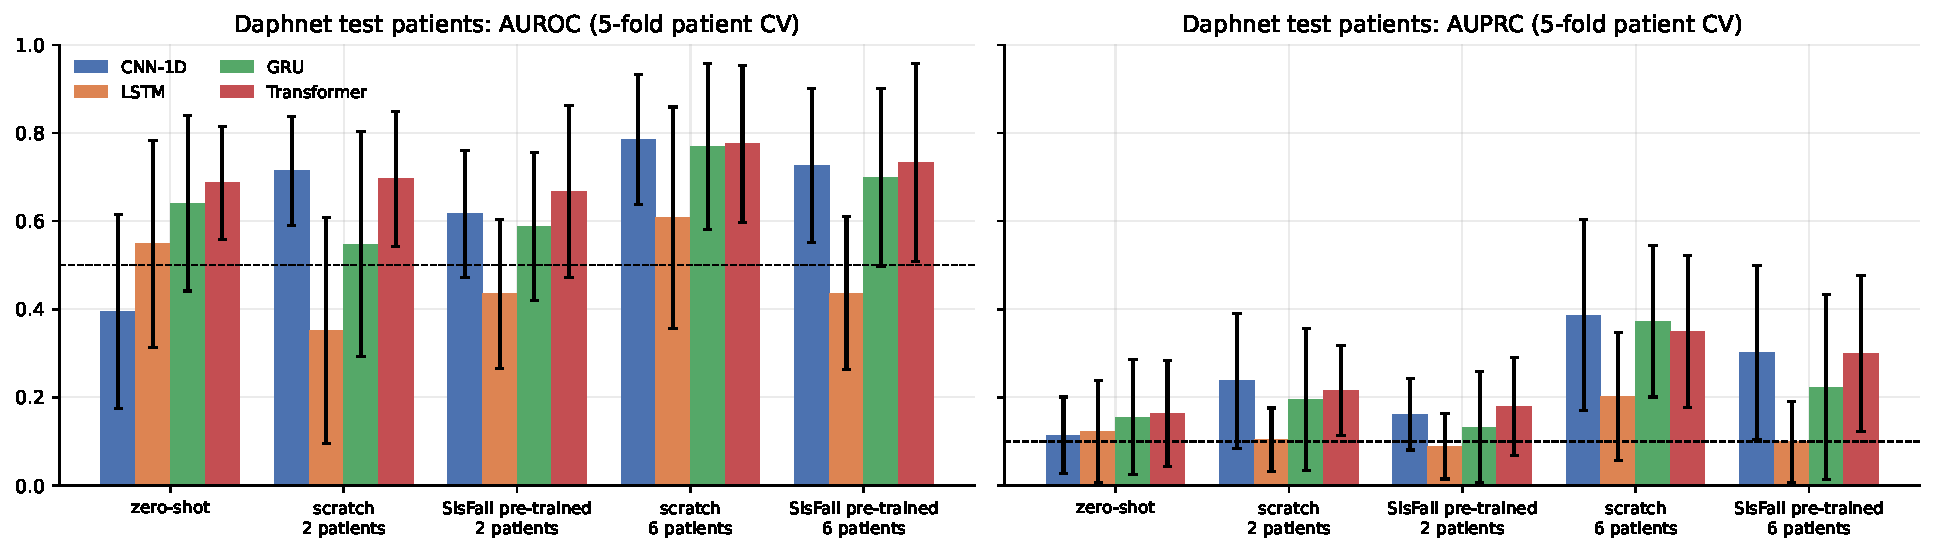
\includegraphics[width=\textwidth]{fig19_target_adaptation}
\caption{Daphnet AUROC and AUPRC on held-out patients (mean $\pm$ std over five folds). In the zero-shot
column the threshold is set on the validation patients of each fold, so its AUROC is computed on a
smaller set of patients than in \Cref{tab:zeroshot}.}
\label{fig:adaptation}
\end{figure}

\section{E4: covariate shift and concept shift in the representations}
\label{sec:e4}

\Cref{tab:shift} and \Cref{fig:shift} examine the penultimate-layer embeddings of the SisFall models
(seed 0).

\paragraph{Covariate shift is large and survives normalisation.} A linear probe separates SisFall ADL
from Daphnet walking with an AUROC of 0.96--0.995 in every space, whichever normalisation is used.
Domain statistics reduce the squared MMD considerably for the LSTM (0.446 $\to$ 0.017) and the
Transformer (0.128 $\to$ 0.024), but the probe accuracy hardly moves: matching moments is not the
same as making the domains indistinguishable. Parkinsonian walking remains recognisable as such
inside representations that were never trained to see it.

\paragraph{Concept shift is visible as orthogonality.} In raw window statistics, the vector from walking
to FoG points in the same direction as the vector from ADL to falls ($\cos=+0.77$): both mean ``more
movement''. In the learned embeddings, the cosine drops to $+0.18$ (CNN-1D), $+0.10$ (LSTM), $-0.03$
(GRU) and $+0.12$ (Transformer). The networks have learned features specific to impacts and discarded
the generic ``agitation'' direction, which is not discriminative on SisFall because jogging, stairs and
stumbling share it. That direction is precisely what distinguishes FoG from walking at the trunk. The
t-SNE maps (\Cref{fig:tsne-emb}) show the same picture: falls form a separate cluster, and Daphnet
walking and FoG windows are interleaved with each other and partly overlap SisFall ADL.

\begin{table}[ht]
\centering
\footnotesize
\caption{Shift between SisFall ADL and Daphnet walking, in input space and in the embedding of each SisFall-trained model: squared MMD, AUROC of a linear domain probe, under source and domain normalisation; and cosine between the fall and FoG class-difference directions.}
\label{tab:shift}
\setlength{\tabcolsep}{4pt}
\begin{adjustbox}{max width=\textwidth}
\begin{tabular}{lccccc}
\toprule
 & \multicolumn{2}{c}{MMD$^2$} & \multicolumn{2}{c}{Domain probe AUROC} & \\
\cmidrule(lr){2-3}\cmidrule(lr){4-5}
Space & source st. & domain st. & source st. & domain st. & $\cos(\Delta_\mathcal{S},\Delta_\mathcal{T})$ \\
\midrule
Input statistics & 0.110 & 0.072 & 0.958 & 0.995 & +0.766 \\
CNN-1D & 0.200 & 0.081 & 0.994 & 0.995 & +0.182 \\
LSTM & 0.446 & 0.017 & 0.989 & 0.975 & +0.096 \\
GRU & 0.097 & 0.074 & 0.993 & 0.981 & -0.030 \\
Transformer & 0.128 & 0.024 & 0.976 & 0.962 & +0.122 \\
\bottomrule
\end{tabular}
\end{adjustbox}
\end{table}

\begin{figure}[ht]
\centering
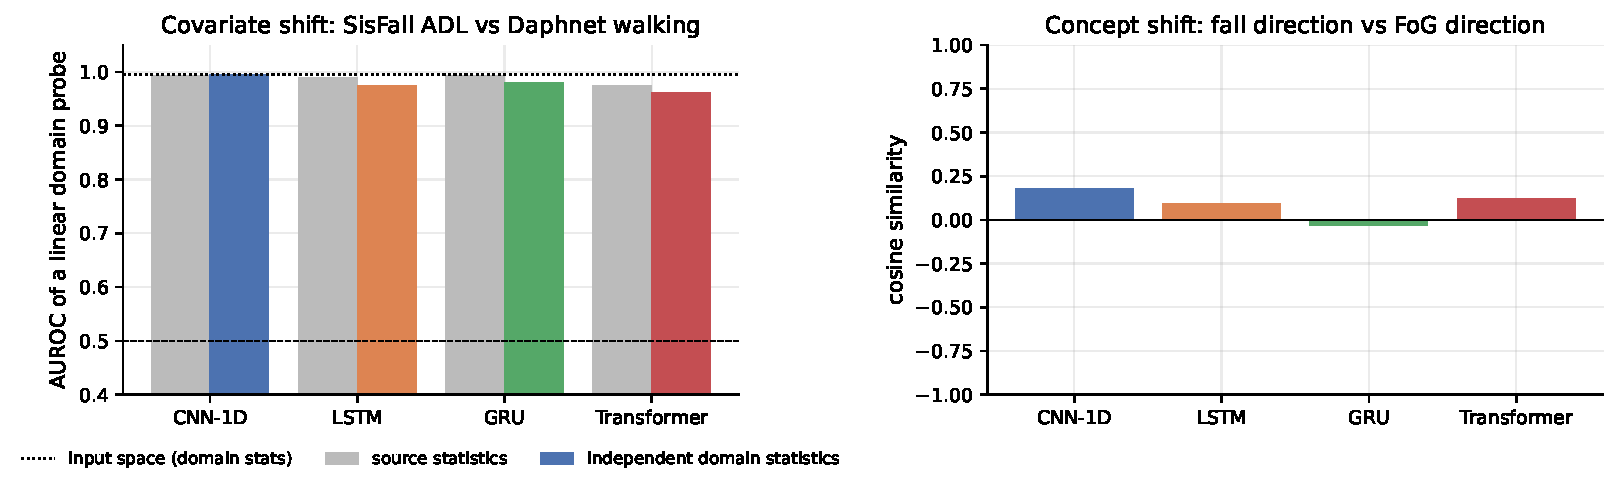
\includegraphics[width=\textwidth]{fig21_shift_decomposition}
\caption{Left: AUROC of a linear probe separating SisFall ADL from Daphnet walking in each model's
embedding (dotted line: input statistics). Right: cosine between the fall--ADL and FoG--walking
class-mean differences in each embedding.}
\label{fig:shift}
\end{figure}

\begin{figure}[ht]
\centering
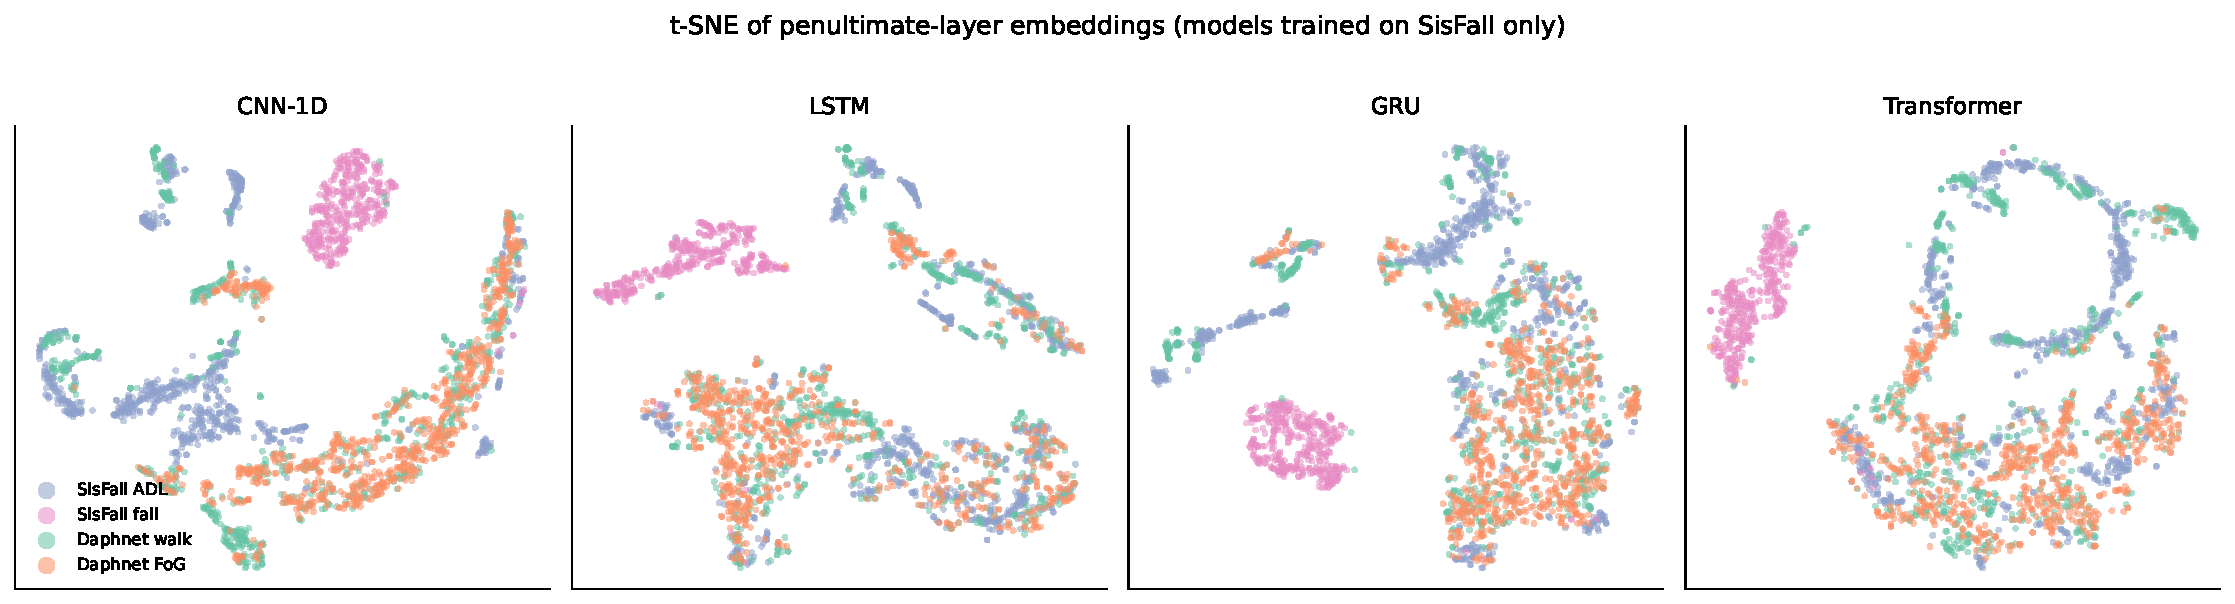
\includegraphics[width=\textwidth]{fig20_embedding_tsne}
\caption{t-SNE of penultimate-layer embeddings for 800 windows per group (SisFall test subjects and
Daphnet).}
\label{fig:tsne-emb}
\end{figure}

\section{Synthesis}
\label{sec:synthesis}

\Cref{fig:overview} gathers every setting. Four observations summarise the study.
\begin{enumerate}
  \item \textbf{In-domain accuracy says nothing about transfer.} All four models are near-perfect on
  SisFall and near chance on Daphnet. Source validation could not even rank configurations by
  transferability.
  \item \textbf{The failure is mostly concept shift.} Normalisation removes part of the covariate shift
  without improving transfer; the learned fall direction is orthogonal to the FoG direction; and fall
  pre-training hurts fine-tuning.
  \item \textbf{Architectures differ more under shift than in-domain, but not enough to matter.} The
  Transformer is the only model whose zero-shot interval excludes chance, and with the GRU it gives the
  best zero-shot ranking. The CNN-1D, worst under zero-shot transfer, is the best model once a few
  patients are labelled. None of these differences survives the patient-level uncertainty.
  \item \textbf{Physics beats transfer.} A 2008 hand-crafted freeze index, or simply the window's
  energy, ranks FoG better than any fall detector, without a single label.
\end{enumerate}

\begin{figure}[ht]
\centering
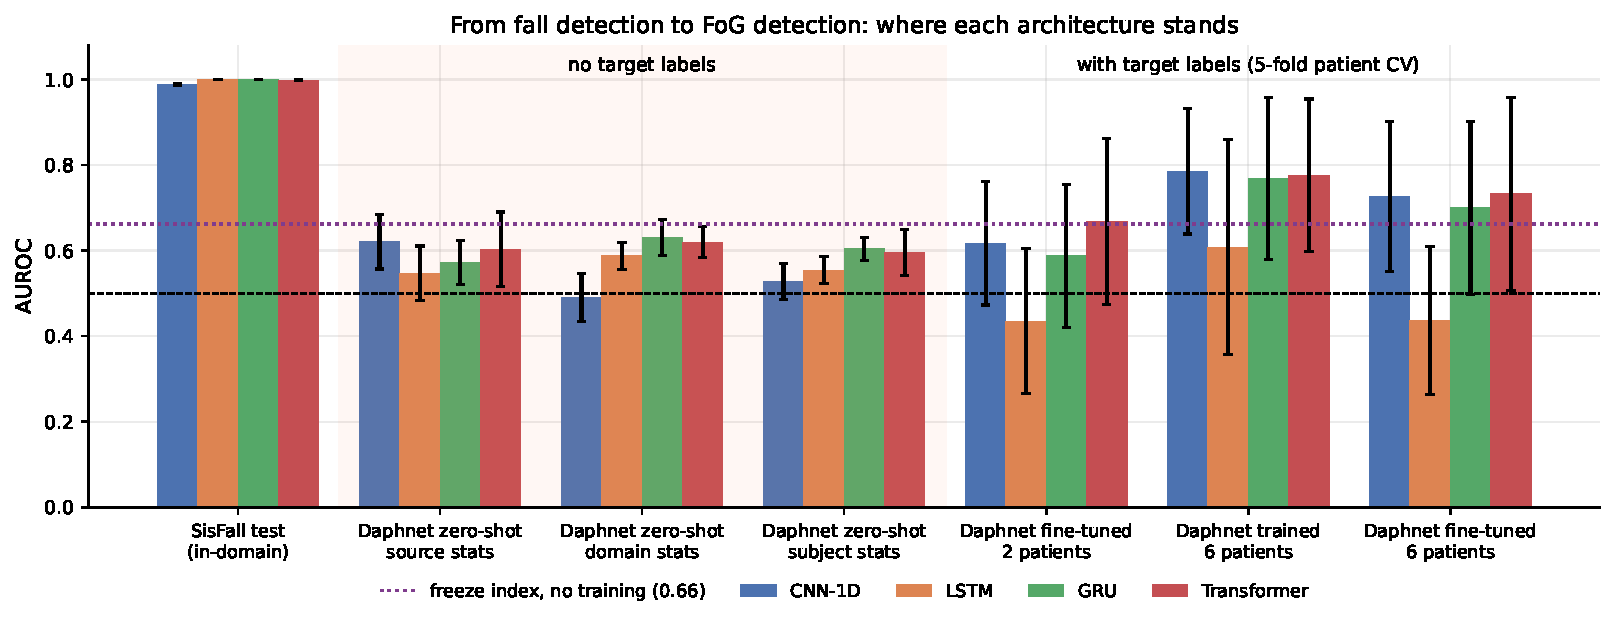
\includegraphics[width=\textwidth]{fig22_overview_auroc}
\caption{AUROC per setting and architecture (error bars: std over seeds for SisFall and zero-shot,
over folds for target-label settings). Dotted line: training-free freeze index.}
\label{fig:overview}
\end{figure}

\section{Limitations}
\label{sec:limitations}

Daphnet contains ten patients, two of whom never freeze, so every target-domain estimate carries wide
intervals; the subject bootstrap makes that explicit, but conclusions about architectures remain
tentative. The trunk sensor is the anatomically fair choice for comparison with SisFall, but it is not
the best place to detect FoG; the ceiling reported in E3 should not be read as the state of the art for
Daphnet, where shank sensors and longer windows are standard. Fall impacts were located automatically
from the signal magnitude, which is reliable for clear impacts but may misplace the event in a few
cushioned falls. SisFall falls were performed on mattresses by healthy volunteers, so even in-domain
results are optimistic for real falls \parencite{bagala2012realfalls}. Training ran on a GPU, whose
recurrent kernels are not bit-exact; re-running inference from the saved checkpoints on a CPU
reproduced every reported metric to four decimals.

\chapter{Conclusion}
\label{ch:conclusion}

\section{Summary}

This study asked whether a deep fall detector trained on healthy volunteers can recognise freezing of
gait in people with Parkinson's disease, and why it cannot. With the confounders removed by
construction, the answers to the four research questions are as follows.

\textbf{RQ1.} On unseen SisFall subjects, CNN-1D, LSTM, GRU and patch Transformer are all excellent
(AUROC 0.988--0.999, 0.7--1.5 false alarms per hour). The recurrent models are marginally ahead,
but no ranking is supported by the subject-level uncertainty. With impact-centred labels, simulated fall
detection is essentially a solved problem, so it is a poor benchmark for choosing an architecture.

\textbf{RQ2.} Zero-shot, the detectors rank FoG only slightly above walking (AUROC 0.49--0.63; 0.65 for the
Transformer seed ensemble, the only interval that excludes chance), and at their validated operating
point they detect essentially no freezing episode while raising 12--23 false alarms per hour of
Parkinsonian walking. A single-line freeze index outperforms all of them.

\textbf{RQ3.} The gap is mostly concept shift. Label-free normalisation reduces the distance between
domains without making them indistinguishable and without improving transfer, and the direction that
the networks use to flag falls is nearly orthogonal to the one that separates FoG from walking.

\textbf{RQ4.} When patients are labelled, fall pre-training is a worse initialisation than random
weights. Trained from scratch on six patients with a trunk sensor, the models reach an AUROC of about
0.78, with the CNN-1D and the Transformer the most data-efficient.

The practical lesson is simple: a monitoring system for Parkinson's disease cannot inherit its notion
of ``abnormal'' from simulated falls. A model that is near-perfect on the source domain can be blind
to the target event, and nothing measured on the source domain warns about it.

\section{Perspectives}

\paragraph{Event-agnostic pre-training.} Fall supervision teaches impact detectors. Self-supervised
objectives on large unlabelled wearable corpora (contrastive or masked reconstruction,
\cite{eldele2021tstcc}) learn representations of movement itself, including the rhythmic structure that
FoG disrupts, and are a better candidate for transfer.

\paragraph{Physics as an inductive bias.} The freeze index beat every network without training. Feeding
spectral features in the locomotion and freeze bands to the models, or constraining the first layers to
behave like band-pass filters, could combine the robustness of the physical prior with the capacity of
learned models.

\paragraph{Personalisation.} Per-patient AUROC varied from 0.26 to 0.85, and zero-shot rankings even
reversed between patients. Few-shot adaptation from a handful of annotated episodes per patient, or
test-time adaptation of normalisation layers \parencite{li2017adabn}, is a natural next step.

\paragraph{Better targets.} Daphnet is small and was recorded in a laboratory protocol designed to
provoke freezing. Larger home-recorded cohorts with both FoG and real falls, and sensors at the shank as
well as the trunk, would make it possible to test whether the conclusions hold outside this setting.


\footnotesize
\printbibliography[heading=bibintoc,title={References}]
\normalsize

\appendix
\chapter{Reproducibility}
\label{app:repro}

\section{Repository layout}

{\footnotesize
\begin{verbatim}
parkinson-domain-shift/
  data/raw/archives/     SisFall_dataset.zip, Daphnet_dataset.zip (untouched)
  data/processed/        windows in g, metadata, scalers, PyTorch tensors
  notebooks/             01-07, executed, with outputs
  src/                   models, training loop, metrics, transforms
  models/<arch>/seed<k>.pt   checkpoints with config, scaler and threshold
  results/figures/       every figure of this report (PNG and PDF)
  results/metrics/       every table of this report (CSV/JSON)
  results/confusion_matrices/
  paper/                 this report and the poster (LaTeX + PDF)
\end{verbatim}
}

\section{Running the pipeline}

The notebooks are executed in order. Notebooks 01, 02, 06 and 07 take a few minutes; 03--05 train
neural networks and are the only expensive steps. Notebooks 03 and 05 write their results row by
row and skip finished runs when restarted, and notebook 04 reloads existing checkpoints, so an
interrupted run can be resumed. The training notebooks were executed on a Colab T4 GPU with
\texttt{colab/RUN\_ON\_COLAB.ipynb}; notebooks 04, 06 and 07 were then re-executed on CPU from the
saved checkpoints (inference only), which reproduced all metrics to four decimals.

\section{Design decisions and the shortcuts they avoid}

\begin{table}[ht]
\centering
\small
\begin{tabular}{p{3.6cm}p{4.4cm}p{5.2cm}}
\toprule
Aspect & Common shortcut & This study \\
\midrule
Fall labels & every window of a fall file & windows centred on the impact ($\pm0.5$\,s), ambiguous ones dropped \\
Sensors & whatever channels are available in each dataset & one waist/trunk accelerometer in both domains, in a V/AP/ML frame \\
Sampling rate & target upsampled to the source rate & source downsampled to 64\,Hz (anti-aliased) \\
Units & raw counts / mg, then z-scored & $g$ in both domains \\
Target windows & across concatenated recordings & inside contiguous valid segments; dropouts removed \\
Scaling & mean / standard deviation & robust (median/IQR), three label-free target variants \\
Training & tuned separately for each model & identical loss, optimiser, batches, seeds and budget \\
Threshold & fixed by hand & $F_2$-optimal on source validation \\
\bottomrule
\end{tabular}
\caption{Design decisions of this study and the simpler choices they replace.}
\label{tab:changes}
\end{table}

\section{Additional figures}

\begin{figure}[H]
\centering
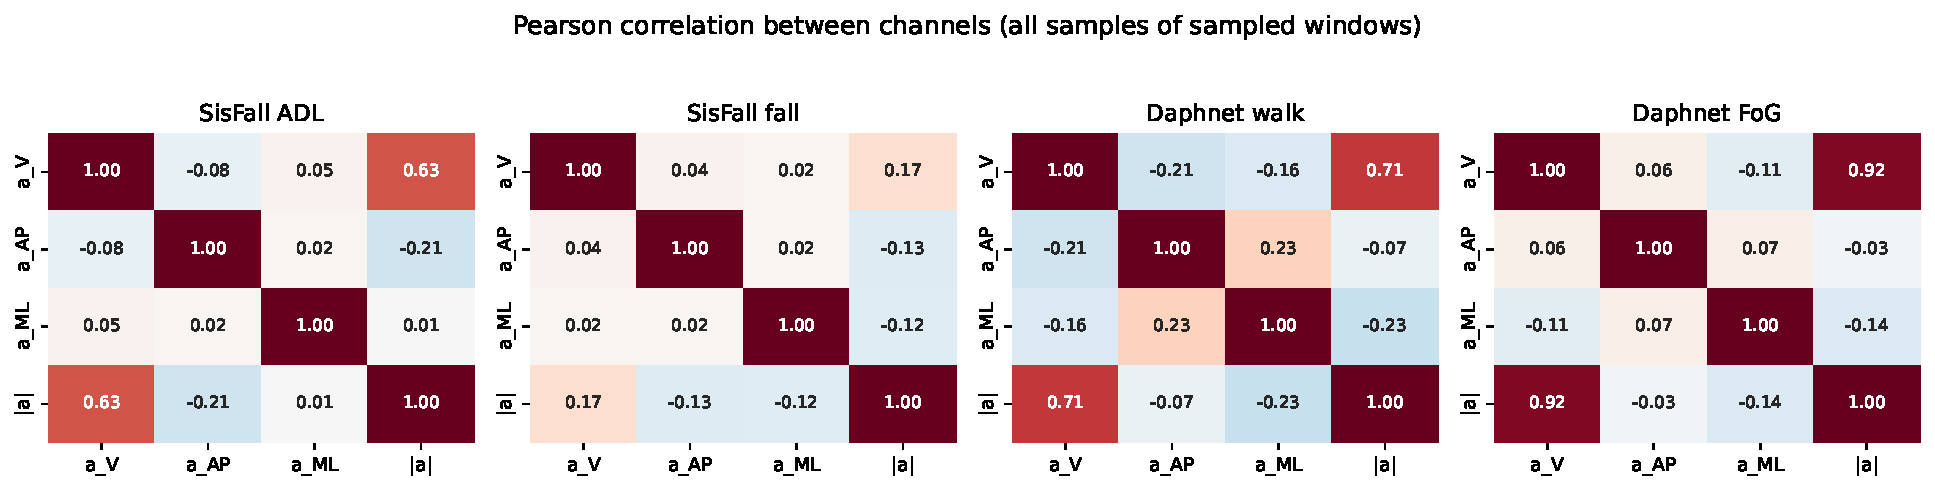
\includegraphics[width=\textwidth]{fig09_channel_correlation}
\caption{Pearson correlation between the four channels, per group.}
\end{figure}

\begin{figure}[H]
\centering
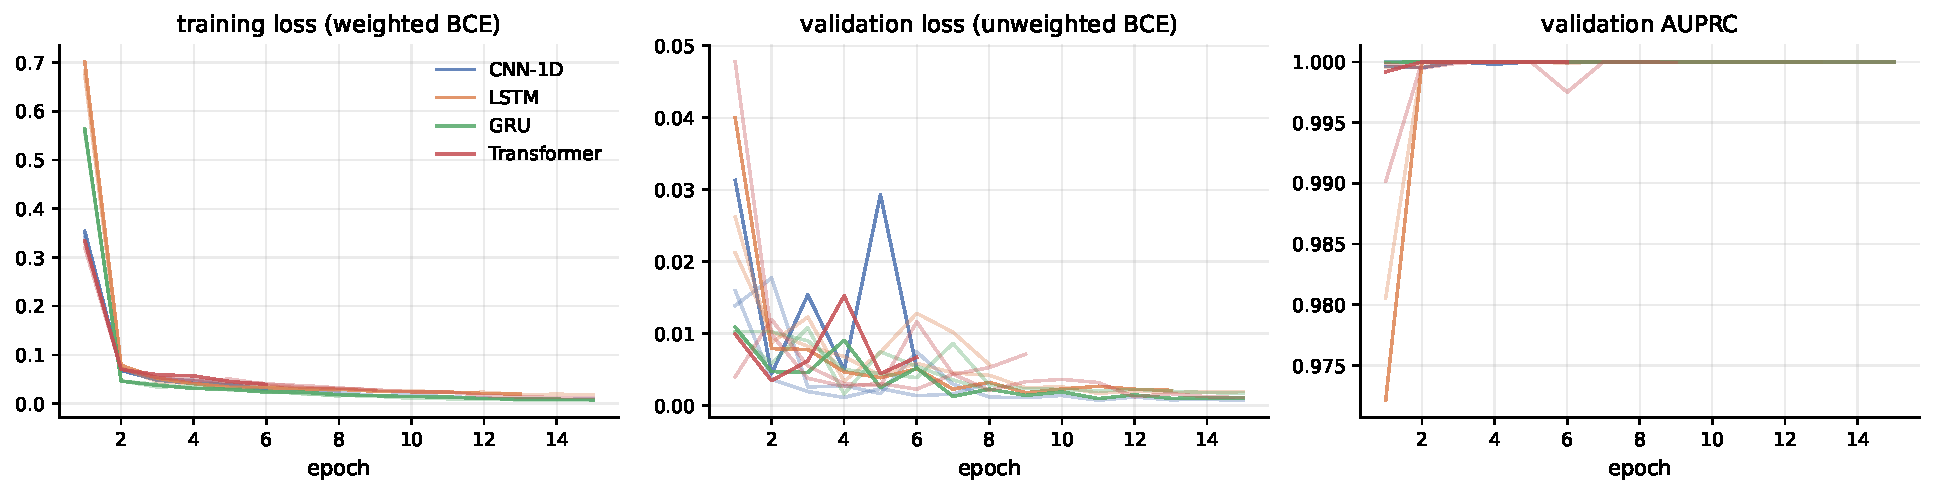
\includegraphics[width=\textwidth]{fig12_learning_curves}
\caption{Learning curves of the final runs (seed 0 opaque, seeds 1--2 transparent).}
\label{fig:curves}
\end{figure}

\begin{figure}[H]
\centering
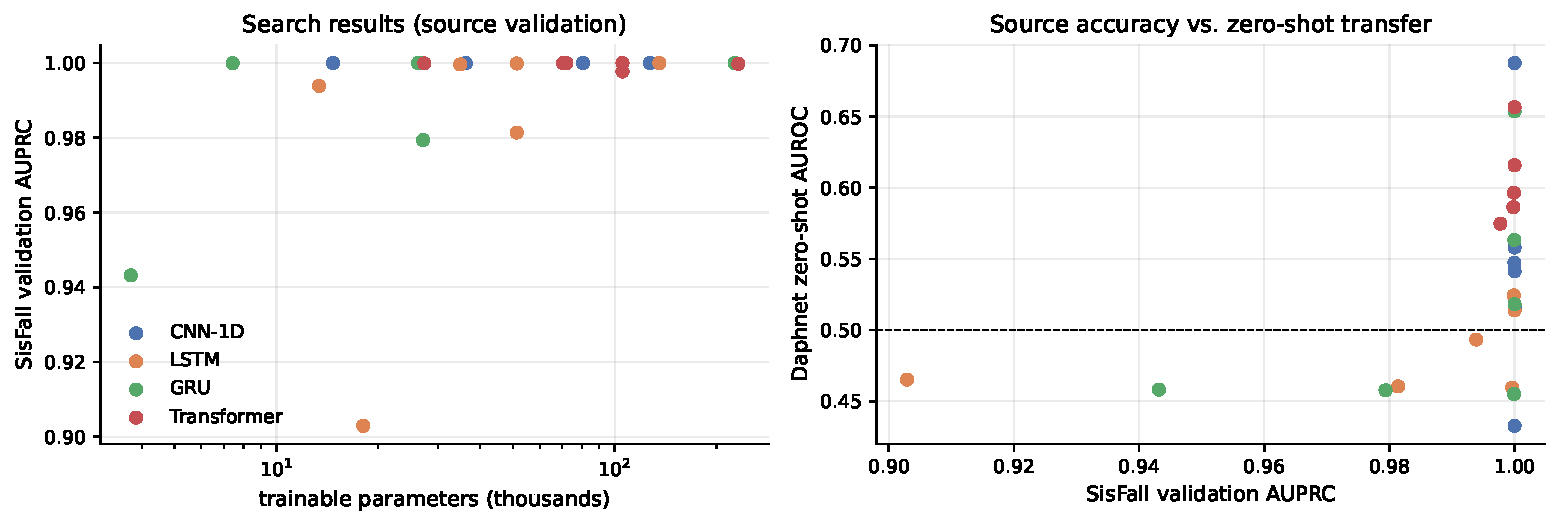
\includegraphics[width=0.95\textwidth]{fig11_hparam_search}
\caption{Hyper-parameter search. Left: validation AUPRC against model size. Right: validation AUPRC
against the Daphnet AUROC that the same configuration would obtain (not used for selection).}
\label{fig:hpsearch}
\end{figure}


\end{document}
